\documentclass[a4paper,12pt]{report}

% Packages nécessaires
\usepackage[french]{babel}
\usepackage[utf8]{inputenc}
\usepackage[T1]{fontenc}
\usepackage{graphicx}
\usepackage{amsmath}
\usepackage{geometry}
\usepackage{float}
\usepackage{hyperref}
\usepackage{tikz}

% Configuration de la géométrie de la page
\geometry{
    a4paper,
    top=2.5cm,
    bottom=2.5cm,
    left=2.5cm,
    right=2.5cm
}

% Informations du titre
\title{\Huge{\textbf{Rapport de Projet de Conception}}\\\Large{Modélisation d'un Drone Quadrirotor avec CATIA V5}}
\author{Votre Nom et Prénom}
\date{\today}

\begin{document}

% Remplacement du \maketitle standard par la page titre personnalisée
\begin{titlepage}
    \begin{center}
        \vspace*{1cm}
        
        \textbf{\LARGE{École d'Ingénieurs}} \\
        \vspace{0.5cm}
        \textbf{\Large{Formation Génie Mécanique}}
        
        \vspace{2cm}
        
        % Image à remplacer par le logo de votre école
        % \includegraphics[width=0.3\textwidth]{images/logo_ecole.png}
        
        \vspace{2cm}
        
        \textbf{\Huge{RAPPORT DE PROJET}}\\
        \vspace{0.5cm}
        \textbf{\LARGE{Conception Assistée par Ordinateur}}\\
        \vspace{1cm}
        \textbf{\huge{Modélisation d'un Drone Quadrirotor avec CATIA V5}}
        
        \vspace{1.5cm}
        
        \begin{tabular}{l l}
            \textbf{Projet:} & Drone Quadrirotor \\
            \textbf{Année académique:} & 2023-2024 \\
        \end{tabular}
        
        \vfill
        
        \begin{tabular}{l l}
            \textbf{Réalisé par:} & [Votre Nom et Prénom] \\
            & [Votre Numéro d'étudiant] \\
            \\
            \textbf{Sous la supervision de:} & [Nom du Professeur] \\
        \end{tabular}
        
        \vspace{1cm}
        
        \begin{center}
            \rule{0.5\textwidth}{0.5pt}
        \end{center}
        
        \vspace{0.5cm}
        
        {\Large{\today}}
        
    \end{center}
\end{titlepage}

\tableofcontents
\newpage

\chapter{Introduction}
\section{Présentation du projet}
Ce rapport présente le travail réalisé dans le cadre du projet de conception utilisant le logiciel CATIA V5. L'objectif était de concevoir un drone quadrirotor complet, incluant sa structure mécanique et ses systèmes de propulsion.

\section{Analyse fonctionnelle du drone}
L'analyse fonctionnelle permet de définir les besoins auxquels le drone doit répondre, en identifiant ses fonctions principales, contraintes et relations avec l'environnement. Cette démarche est essentielle pour garantir que la conception réponde aux attentes des utilisateurs et aux exigences du cahier des charges.

\subsection{Bête à cornes}
La bête à cornes permet de visualiser le besoin fondamental auquel répond le drone :

\begin{itemize}
    \item \textbf{Qui utilise le drone ?} \quad Utilisateur (opérateur, client)
    \item \textbf{Sur quoi agit-il ?} \quad L'environnement (air, sol, objets à observer ou transporter)
    \item \textbf{Dans quel but ?} \quad Réaliser des missions de prise de vue, de surveillance, de transport léger, etc.
\end{itemize}

% --- Début de la figure Bête à cornes ---
\begin{figure}[H]
    \centering
    \begin{tikzpicture}[node distance=2cm, every node/.style={font=\sffamily}]
        % Les trois branches
        \node (but) [draw, rectangle, minimum width=5cm, minimum height=1cm, fill=gray!10] {\textbf{Dans quel but ?}\\Réaliser des missions (prise de vue, surveillance, transport)};
        \node (objet) [left=of but, draw, rectangle, minimum width=4cm, minimum height=1cm, fill=gray!10] {\textbf{Sur quoi ?}\\L'environnement};
        \node (qui) [right=of but, draw, rectangle, minimum width=4cm, minimum height=1cm, fill=gray!10] {\textbf{Qui ?}\\Utilisateur};
        % Les cornes
        \draw[thick] (objet.east) -- (but.west);
        \draw[thick] (qui.west) -- (but.east);
        % Le corps
        \node (drone) [below=1.5cm of but, draw, rectangle, minimum width=4cm, minimum height=1cm, fill=blue!10] {\textbf{Drone quadrirotor}};
        \draw[thick] (but.south) -- (drone.north);
    \end{tikzpicture}
    \caption{Bête à cornes du drone quadrirotor}
    \label{fig:bete_a_cornes}
\end{figure}
% --- Fin de la figure Bête à cornes ---

\subsection{Diagramme des fonctions (FAST simplifié)}
\begin{itemize}
    \item \textbf{FP1 : Se déplacer dans l'espace aérien} (fonction principale)
    \item \textbf{FP2 : Transporter une charge utile} (caméra, capteur, petit colis)
    \item \textbf{FP3 : Transmettre des informations} (vidéo, données de capteurs)
    \item \textbf{FC1 : Être alimenté électriquement} (batterie, gestion de l'énergie)
    \item \textbf{FC2 : Être piloté à distance} (télécommande, interface utilisateur)
    \item \textbf{FC3 : Assurer la sécurité des personnes et des biens} (protection, arrêt d'urgence)
    \item \textbf{FC4 : Résister aux conditions extérieures} (vent, pluie, chocs)
\end{itemize}

\subsection{Contraintes}
\begin{itemize}
    \item \textbf{Réglementation} : Respecter les normes de sécurité et d'usage des drones civils
    \item \textbf{Poids} : Limiter la masse pour optimiser l'autonomie
    \item \textbf{Autonomie} : Assurer un temps de vol suffisant pour la mission
    \item \textbf{Robustesse} : Résister aux chocs et aux vibrations
    \item \textbf{Facilité d'utilisation} : Prise en main intuitive, maintenance aisée
    \item \textbf{Coût} : Rester dans un budget raisonnable
\end{itemize}

Cette analyse fonctionnelle structure la démarche de conception et oriente les choix techniques détaillés dans la suite du rapport.

\subsection{Contexte et objectifs}
Les drones quadrirotors sont des aéronefs à décollage et atterrissage verticaux (VTOL) qui connaissent un développement considérable ces dernières années. Ils sont utilisés dans de nombreux domaines comme la photographie aérienne, l'inspection de structures, la surveillance, la recherche scientifique ou les loisirs.

Notre projet s'inscrit dans le cadre d'une formation en ingénierie mécanique et vise plusieurs objectifs:
\begin{itemize}
    \item Conception d'un drone quadrirotor fonctionnel et réaliste
    \item Application des principes de conception mécanique
    \item Maîtrise des outils de CAO avancés de CATIA V5
    \item Respect des contraintes de fabrication industrielle
    \item Optimisation des performances (légèreté, rigidité, aérodynamique)
\end{itemize}

\subsection{Cahier des charges}
Le drone devait répondre aux spécifications suivantes:
\begin{itemize}
    \item \textbf{Dimensions}: Envergure maximale de 400mm (entre axes des moteurs opposés)
    \item \textbf{Masse}: Masse totale n'excédant pas 500g (structure seule)
    \item \textbf{Propulsion}: Quatre moteurs brushless avec hélices de 120mm de diamètre
    \item \textbf{Structure}: Résistante aux vibrations et aux contraintes de vol
    \item \textbf{Ergonomie}: Système de prise en main ergonomique
    \item \textbf{Modularité}: Possibilité d'ajouter des accessoires (caméra, capteurs)
    \item \textbf{Fabrication}: Conception compatible avec les procédés d'injection plastique et d'usinage CNC
\end{itemize}

\subsection{Démarche adoptée}
Pour réaliser ce projet, nous avons suivi une méthodologie structurée:
\begin{enumerate}
    \item Étude de l'existant et analyse des solutions techniques
    \item Conception préliminaire des différentes pièces
    \item Validation technique par simulation numérique
    \item Conception détaillée des composants
    \item Assemblage virtuel et vérification des interférences
    \item Réalisation des dessins de définition et d'ensemble
    \item Analyse critique et proposition d'améliorations
\end{enumerate}

\section{Outils utilisés}
Pour réaliser ce projet, nous avons principalement utilisé CATIA V5, un logiciel de conception assistée par ordinateur (CAO) développé par Dassault Systèmes. Ce logiciel nous a permis de modéliser les différentes pièces, de réaliser les assemblages et de générer les dessins techniques.

\subsection{Modules CATIA utilisés}
Plusieurs modules de CATIA V5 ont été mobilisés pour ce projet:
\begin{itemize}
    \item \textbf{Part Design}: Pour la modélisation 3D des pièces
    \item \textbf{Assembly Design}: Pour l'assemblage des composants
    \item \textbf{Drafting}: Pour la création des dessins techniques
    \item \textbf{DMU Kinematics}: Pour la simulation des mouvements
    \item \textbf{Generative Shape Design}: Pour la création de surfaces complexes (hélices)
    \item \textbf{Analysis \& Simulation}: Pour les vérifications mécaniques simples
\end{itemize}

\subsection{Autres ressources techniques}
En complément de CATIA V5, nous avons utilisé:
\begin{itemize}
    \item Bibliothèque de matériaux pour les propriétés physiques
    \item Normes ISO pour les cotations et tolérances
    \item Documentation technique sur les moteurs brushless et hélices
    \item Guides de conception pour l'injection plastique
\end{itemize}

\begin{figure}[H]
    \centering
    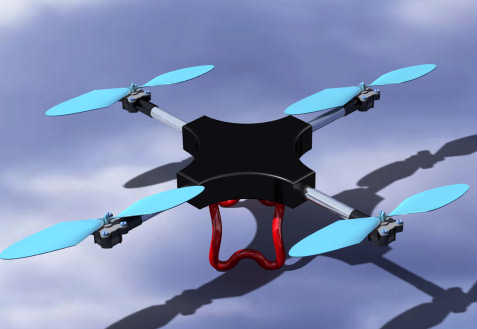
\includegraphics[width=0.8\textwidth]{images/drone_apercu.png}
    \caption{Aperçu du drone quadrirotor conçu dans ce projet}
    \label{fig:drone_apercu}
\end{figure}

Le rapport qui suit détaille l'ensemble du processus de conception, depuis la modélisation des pièces individuelles jusqu'à l'assemblage complet, en passant par les dessins techniques et l'analyse critique du projet.

\chapter{Conception des pièces}
\section{Liste des pièces modélisées}
Dans ce projet, nous avons modélisé les pièces suivantes:
\begin{itemize}
    \item Pièce 1: Châssis central (corps principal)
    \item Pièce 2: Bras de support des moteurs (4 pièces)
    \item Pièce 3: Supports de moteur (4 pièces, fixés aux extrémités des bras)
    \item Pièce 4: Hélices (4 pièces, de couleur bleue)
    \item Pièce 5: Moteurs brushless (4 pièces)
    \item Pièce 6: Support d'attache (en rouge)
    \item Pièce 7: Éléments de fixation (vis et écrous pour l'assemblage)
    \item Pièce 8: Capot de protection électronique
    % Ajoutez d'autres pièces selon votre projet
\end{itemize}

\section{Procédures de modélisation}
\subsection{Modélisation du châssis central}
Pour modéliser le châssis central du drone, nous avons suivi les étapes suivantes:
\begin{enumerate}
    \item \textbf{Création d'une esquisse sur le plan XY}:
    \begin{itemize}
        \item Dessin d'un octogone régulier comme base du châssis
        \item Application des contraintes de symétrie par rapport aux axes
        \item Cotation du diamètre extérieur à 160mm
    \end{itemize}
    
    \begin{figure}[H]
        \centering
        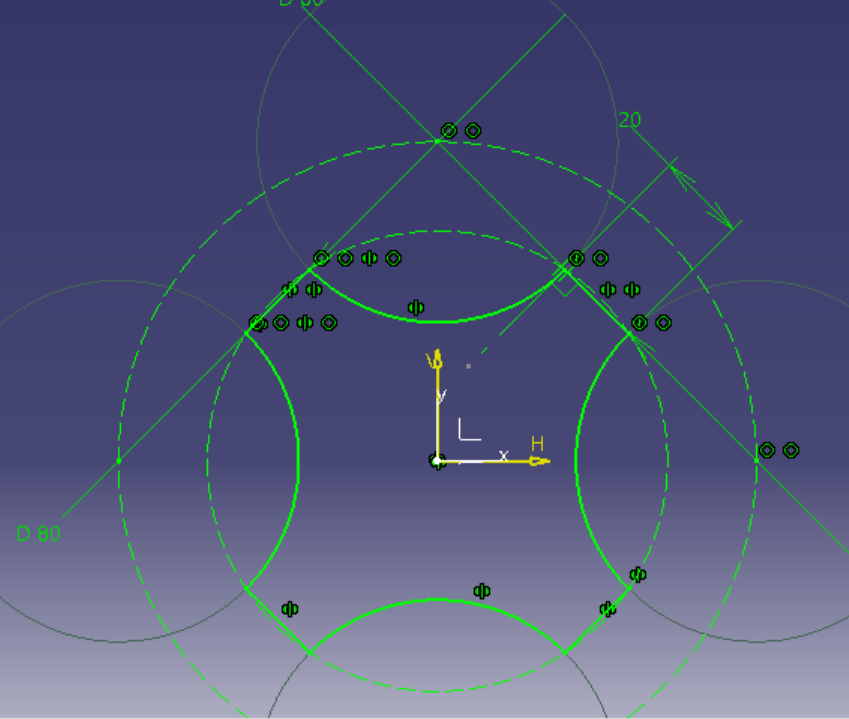
\includegraphics[width=0.8\textwidth]{images/esquisse_chassis_central.png}
        \caption{Esquisse 2D du châssis central avec les contraintes géométriques}
        \label{fig:esquisse_chassis}
    \end{figure}
    
    \item \textbf{Extrusion (Pad) de l'esquisse}:
    \begin{itemize}
        \item Extrusion de 20mm dans la direction Z positif
    \end{itemize}
    
    \begin{figure}[H]
        \centering
        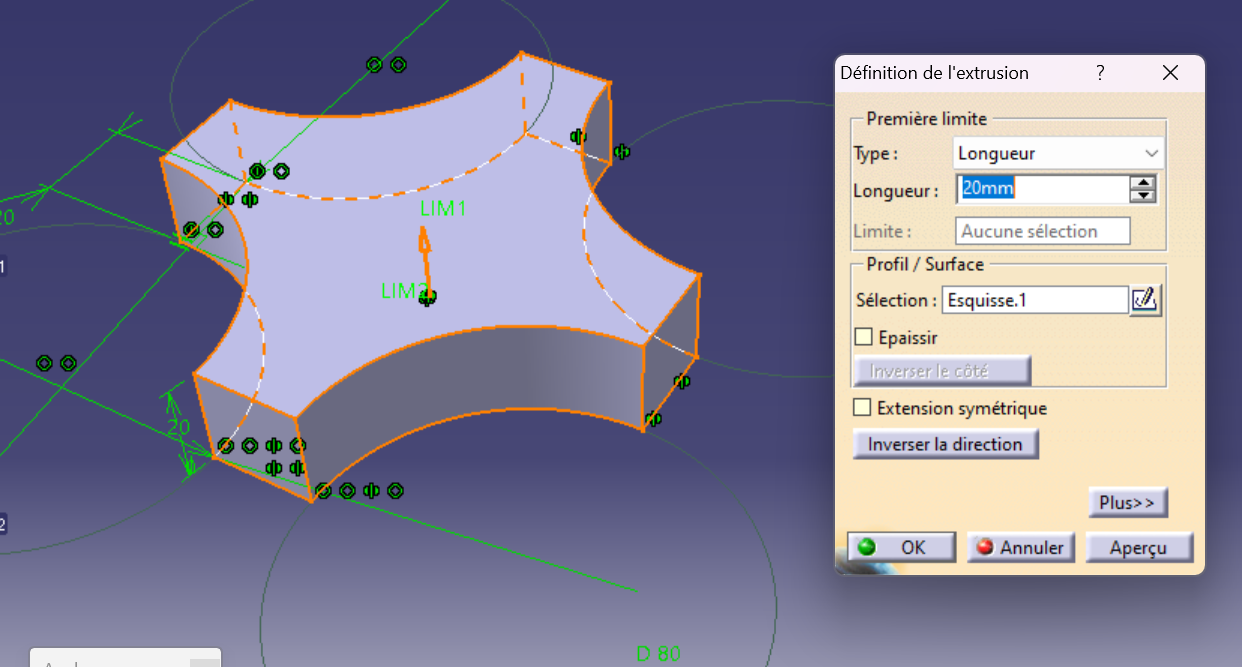
\includegraphics[width=0.8\textwidth]{images/extrusion_chassis_central.png}
        \caption{Opération d'extrusion (Pad) du châssis central de 20mm}
        \label{fig:extrusion_chassis}
    \end{figure}
    
    \item \textbf{Création d'un trou taraudé}:
    \begin{itemize}
        \item Définition d'un trou taraudé M8 sur la face avant du châssis
        \item Profondeur du trou: 10mm
        \item Type de taraudage: Métrique à pas épais
        \item Diamètre avant trou: M8 (7mm)
        \item Profondeur du taraudage: 10mm 
    \end{itemize}
    
    \begin{figure}[H]
        \centering
        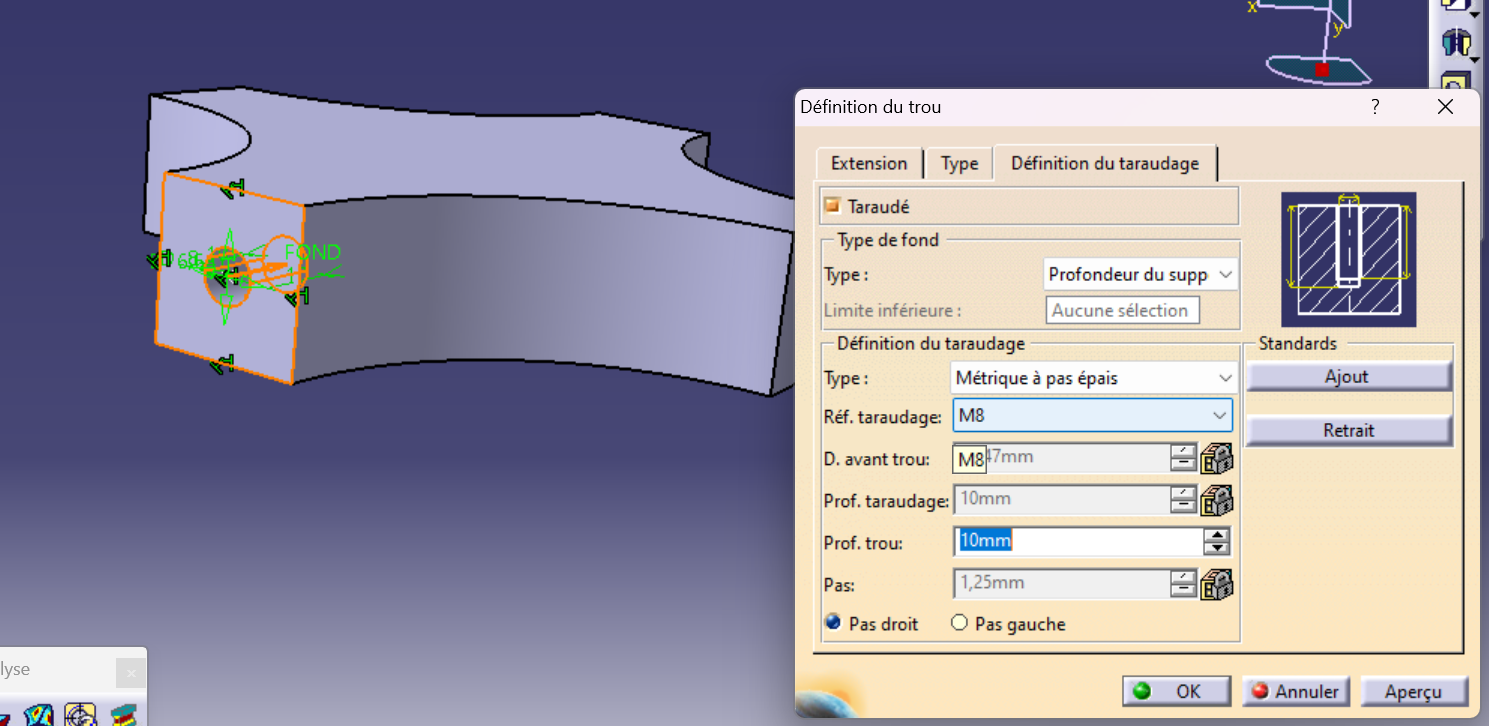
\includegraphics[width=0.8\textwidth]{images/trou_taraude_chassis.png}
        \caption{Création d'un trou taraudé M8 dans le châssis central}
        \label{fig:trou_taraude}
    \end{figure}
    
    \item \textbf{Création d'une répétition circulaire}:
    \begin{itemize}
        \item Application d'un pattern circulaire (Circular Pattern) du trou taraudé
        \item Nombre d'instances: 4
        \item Espacement angulaire: 90 degrés (360° divisé en 4 instances)
        \item Référence axiale: axe central du châssis
        \item Composant à copier: trou.1 
    \end{itemize}
    
    \begin{figure}[H]
        \centering
        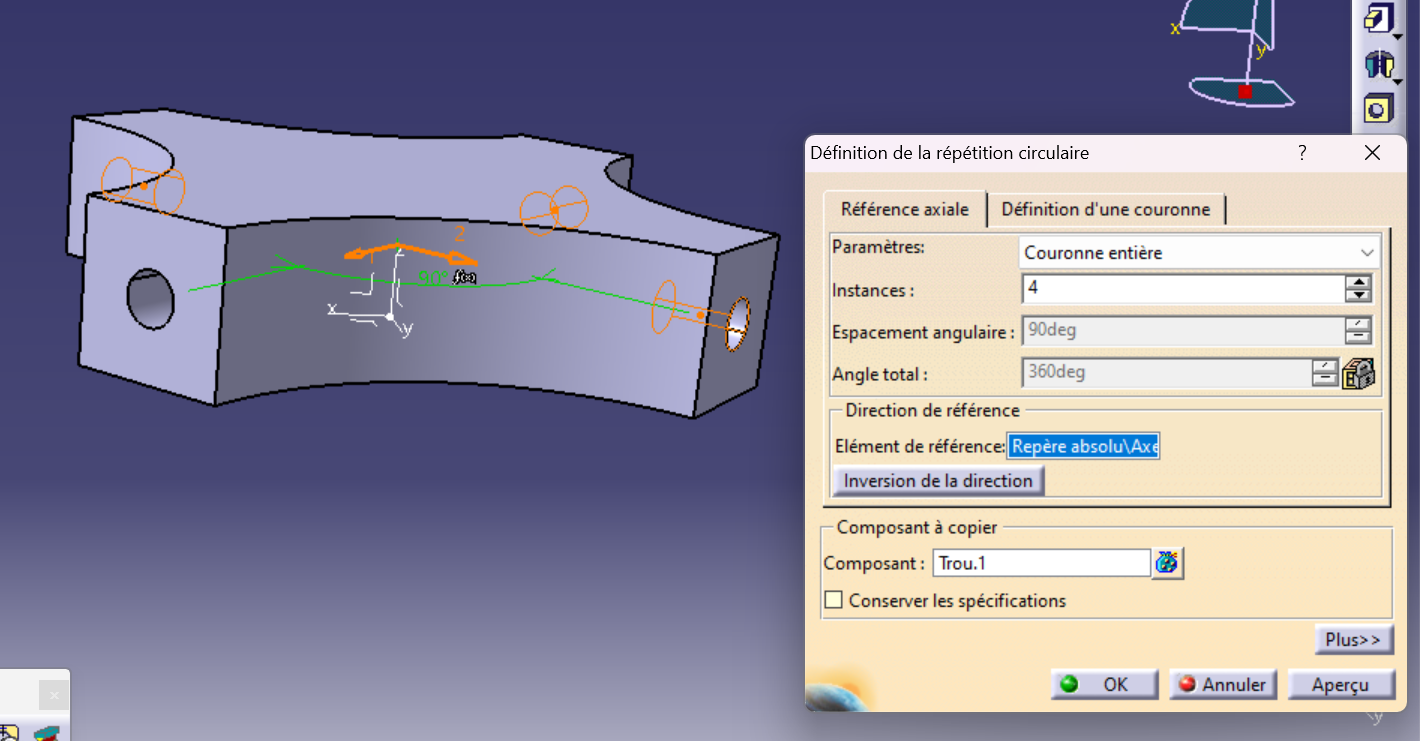
\includegraphics[width=0.8\textwidth]{images/repetition_circulaire_trou.png}
        \caption{Répétition circulaire des trous taraudés M8 à 90° d'intervalle}
        \label{fig:repetition_circulaire}
    \end{figure}
    
    \item \textbf{Application de congés}:
    \begin{itemize}
        \item Utilisation de la fonction Congé (Fillet) pour adoucir les arêtes
        \item Rayon du congé: 2mm
        \item Sélection des arêtes extérieures du châssis (2 éléments)
        \item Mode de sélection: Tangence
    \end{itemize}
    
    \begin{figure}[H]
        \centering
        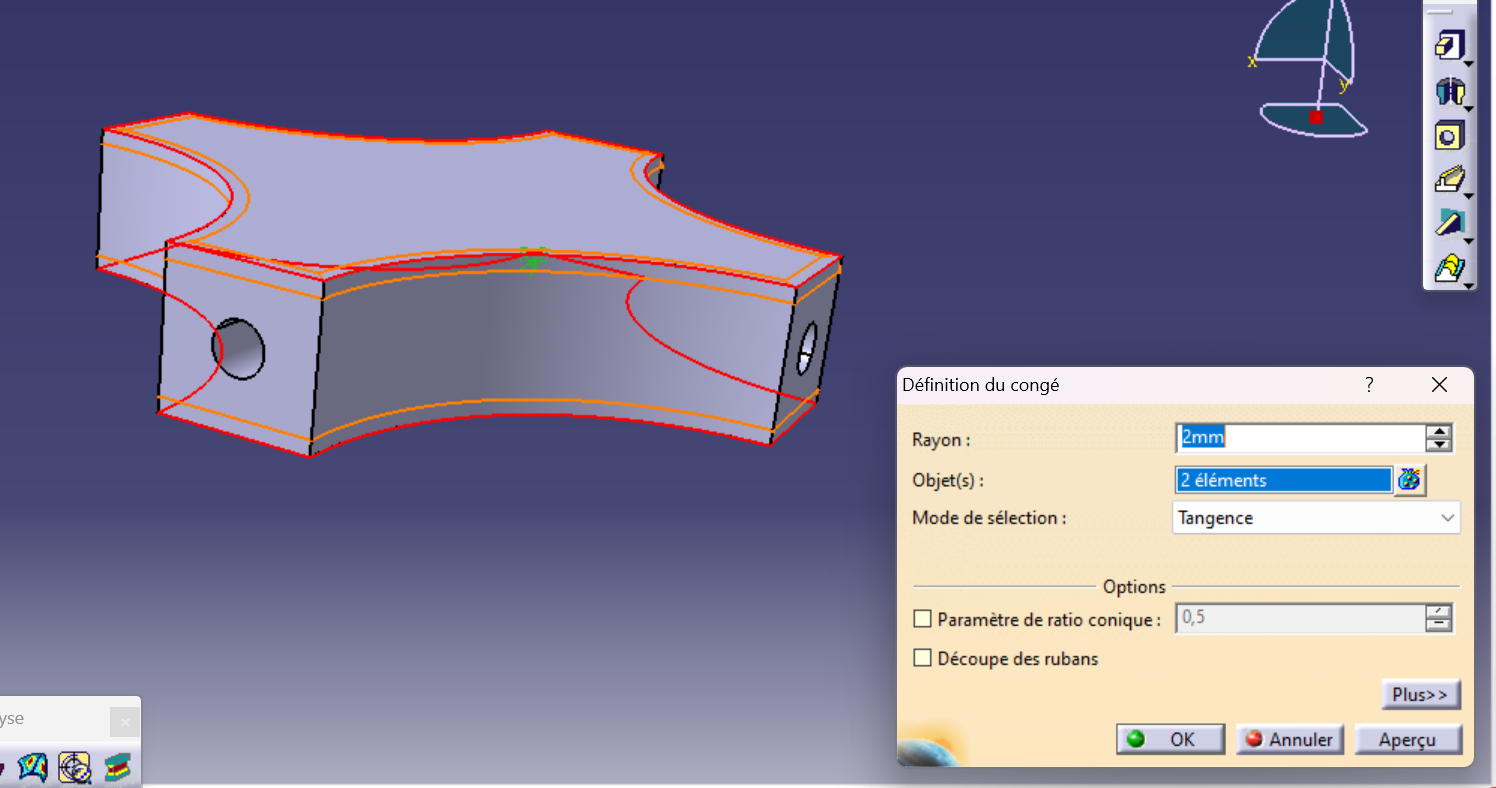
\includegraphics[width=0.8\textwidth]{images/conge_chassis.png}
        \caption{Application de congés de rayon 2mm sur les arêtes du châssis}
        \label{fig:conge_chassis}
    \end{figure}
    
    \item \textbf{Création de poches pour la fixation des pieds}:
    \begin{itemize}
        \item Création d'une nouvelle esquisse (Esquisse.4) sur la face supérieure du châssis
        \item Dessin des contours pour les emplacements des fixations des pieds
        \item Utilisation de la fonction Poche (Pocket) pour creuser ces emplacements
        \item Profondeur de la poche: 6mm
        \item Type: Longueur (type de limite standard)
    \end{itemize}
    
    \begin{figure}[H]
        \centering
        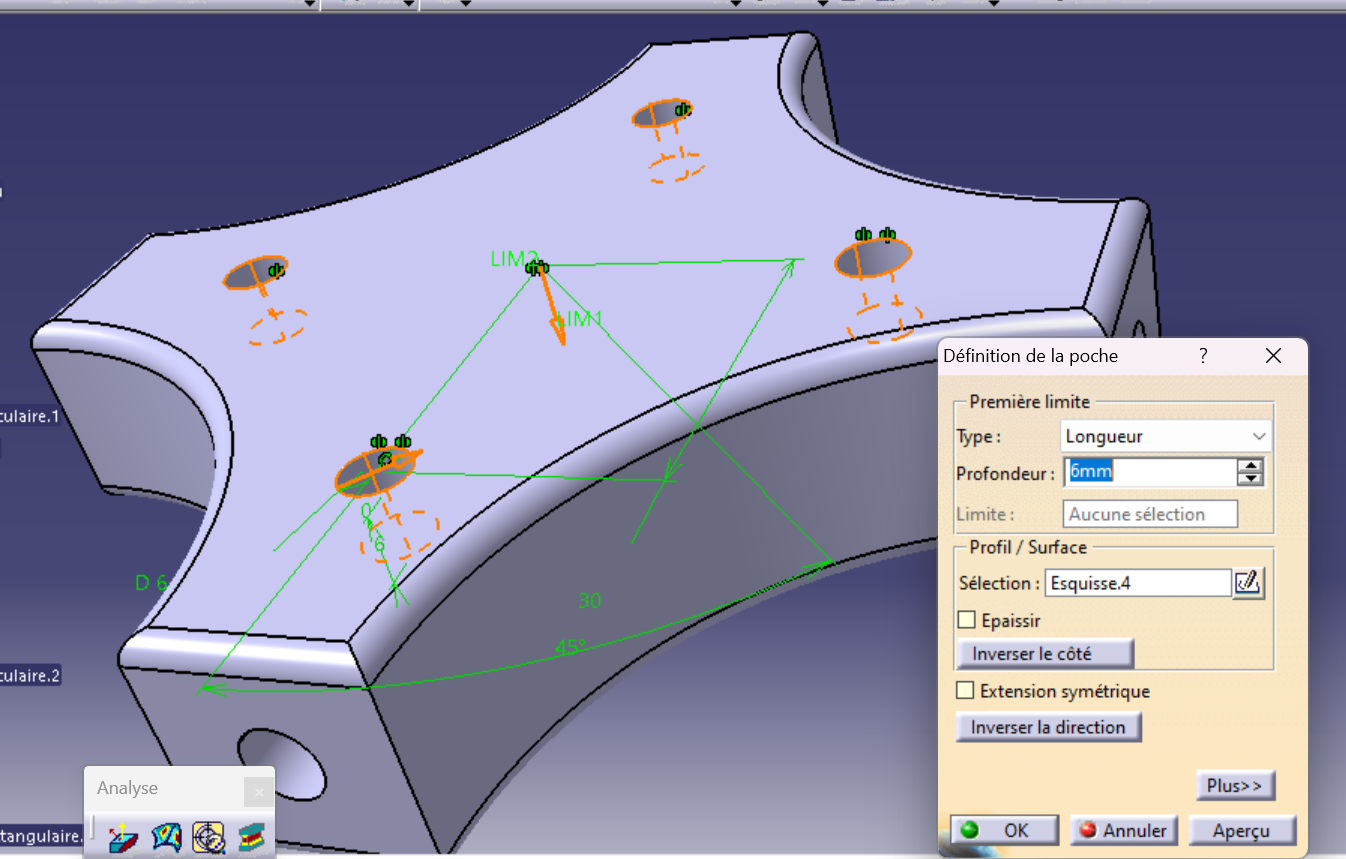
\includegraphics[width=0.8\textwidth]{images/poche_fixation_pieds.png}
        \caption{Création des poches pour la fixation des pieds du drone}
        \label{fig:poche_pieds}
    \end{figure}
    
    \item \textbf{Création de la poche centrale pour l'électronique}:
    \begin{itemize}
        \item Création d'une nouvelle esquisse (Esquisse.5) au centre du châssis
        \item Dessin d'une forme ovale/elliptique pour optimiser l'espace disponible
        \item Utilisation de la fonction Poche (Pocket) pour créer le logement des composants
        \item Type de limite: Jusqu'au suivant
        \item Décalage: -4mm pour laisser une épaisseur suffisante au fond du châssis
    \end{itemize}
    
    \begin{figure}[H]
        \centering
        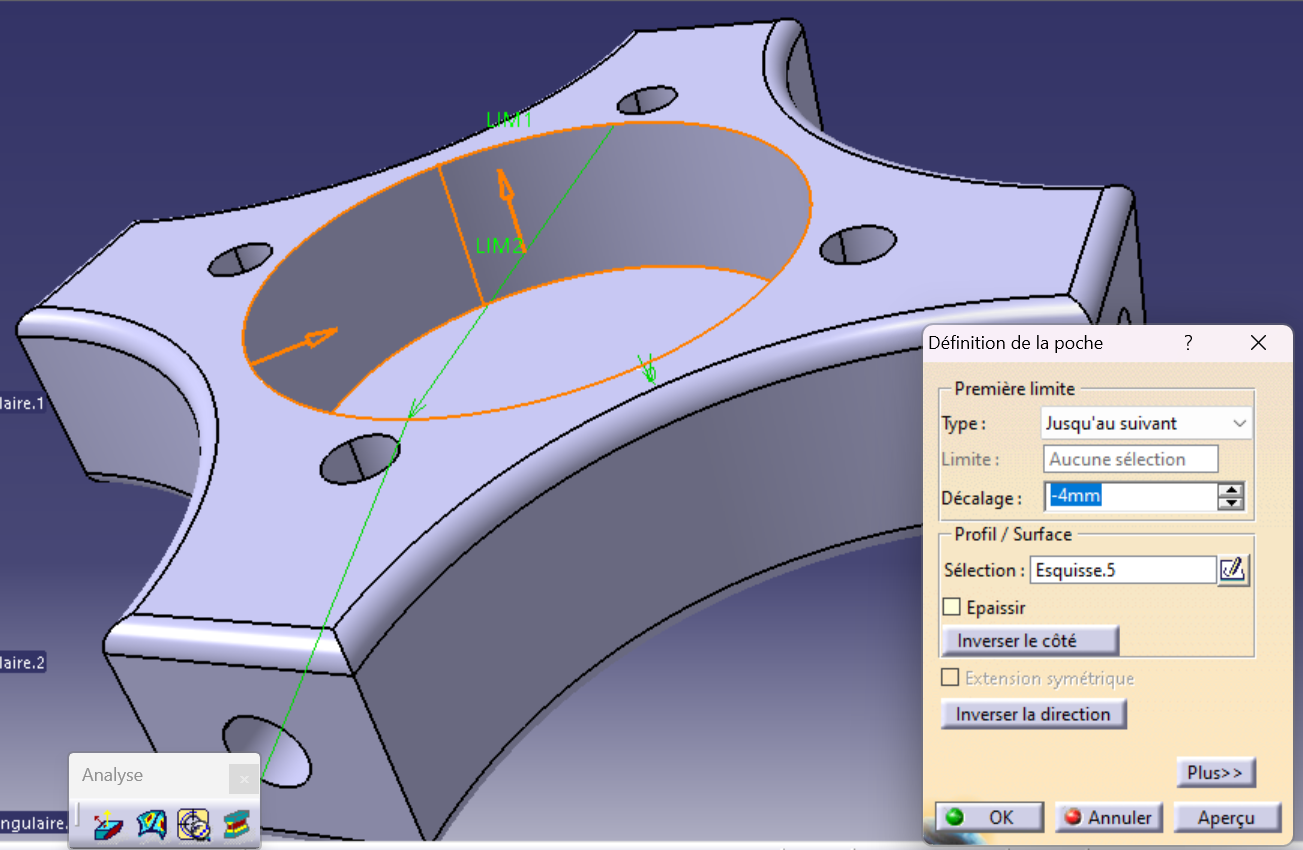
\includegraphics[width=0.8\textwidth]{images/poche_electronique.png}
        \caption{Création de la poche centrale pour les composants électroniques et de contrôle}
        \label{fig:poche_electronique}
    \end{figure}
    
    \item \textbf{Création des nervures de renforcement}:
    \begin{itemize}
        \item Création d'une nouvelle esquisse (Esquisse.6) sur la face inférieure de la poche centrale
        \item Dessin d'un motif de nervures parallèles pour le renforcement structurel
        \item Utilisation de la fonction Extrusion (Rib/Nervure) pour créer les éléments de renfort
        \item Première limite: Type "Jusqu'au suivant" avec décalage de 0mm
        \item Seconde limite: Type "Longueur" avec valeur -14mm (vers le bas)
        \item Épaississement de 1mm pour les nervures
        \item Option "Perpendiculaire au contour" sélectionnée
    \end{itemize}
    
    \begin{figure}[H]
        \centering
        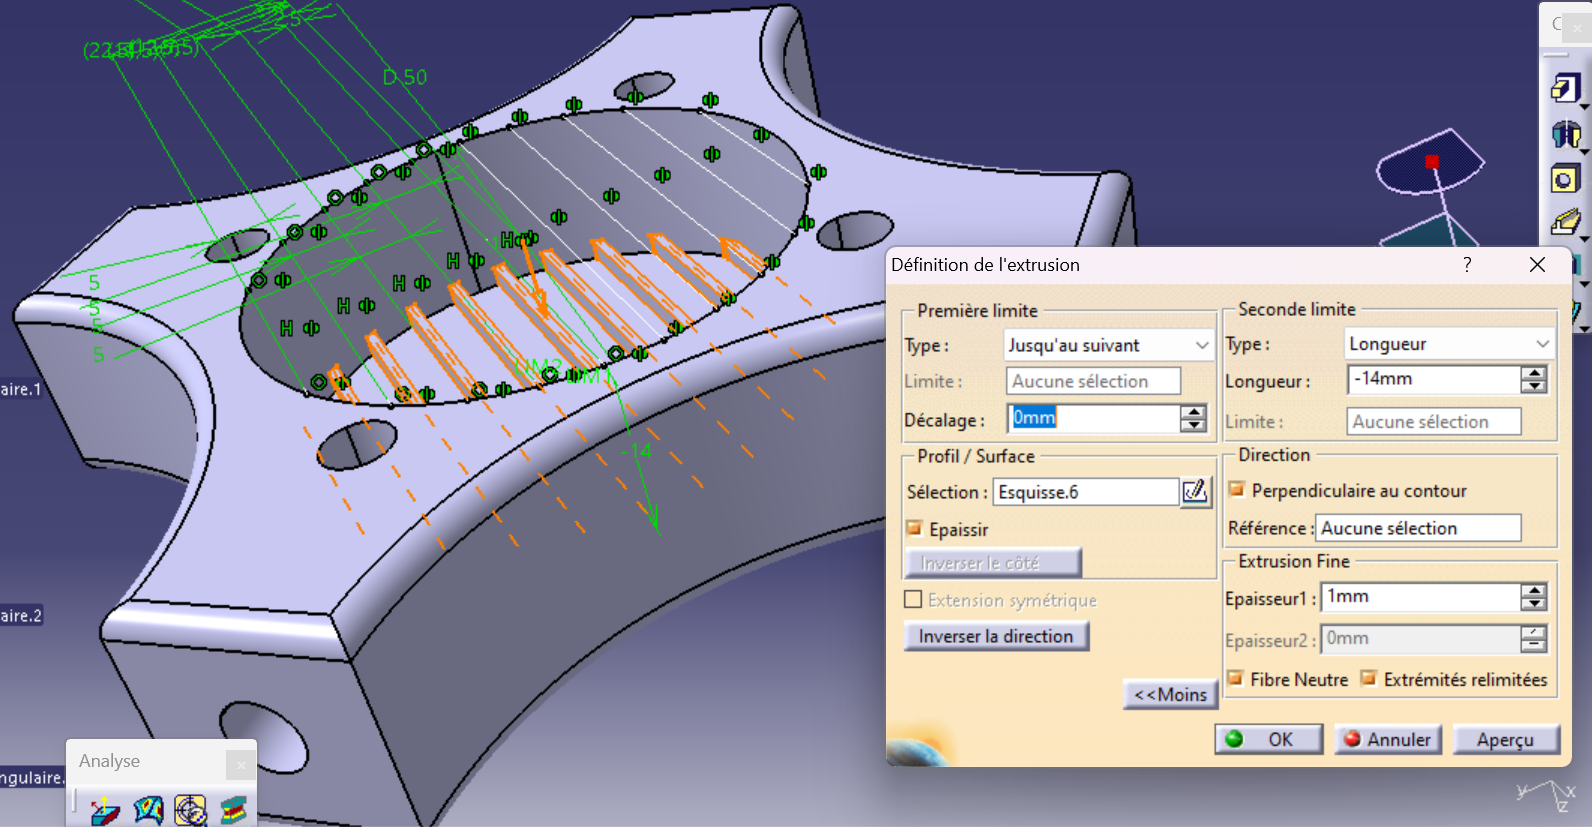
\includegraphics[width=0.8\textwidth]{images/nervures_renforcement.png}
        \caption{Création des nervures de renforcement par extrusion}
        \label{fig:nervures_renforcement}
    \end{figure}
    
    \item \textbf{Répétition circulaire des nervures}:
    \begin{itemize}
        \item Application d'un pattern circulaire (Circular Pattern) aux nervures de renforcement
        \item Composant à copier: Extrusion.2 (ensemble des nervures initiales)
        \item Nombre d'instances: 2
        \item Espacement angulaire: 90 degrés
        \item Angle total: 90 degrés (pour une disposition orthogonale)
        \item Élément de référence: Repère absolu\Axe
        \item Création d'un motif en quadrillage pour un renforcement optimal
    \end{itemize}
    
    \begin{figure}[H]
        \centering
        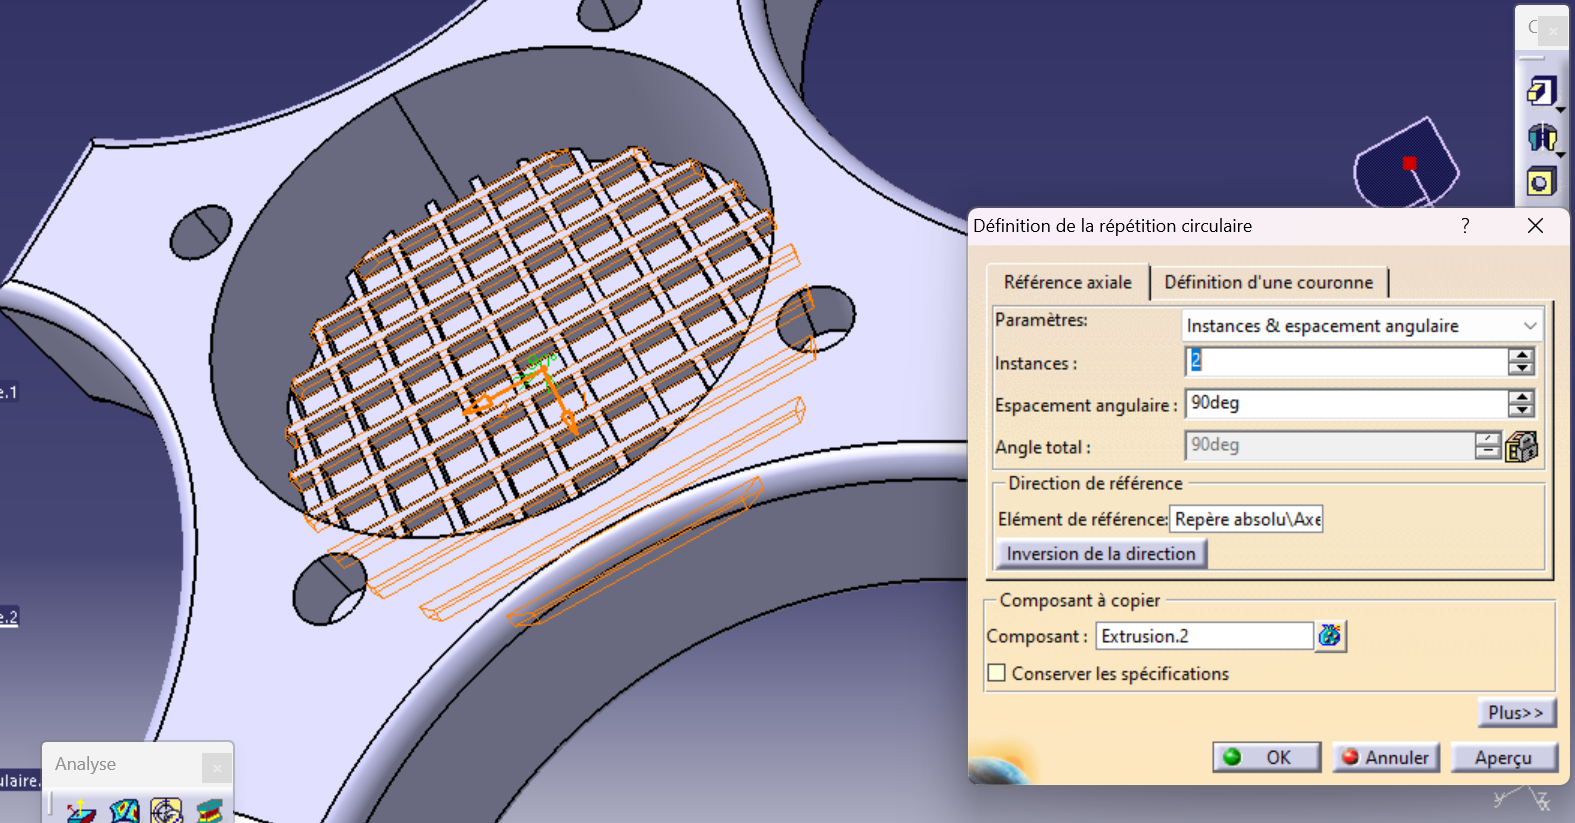
\includegraphics[width=0.8\textwidth]{images/repetition_nervures.png}
        \caption{Répétition circulaire des nervures formant un quadrillage de renforcement}
        \label{fig:repetition_nervures}
    \end{figure}
    
    \item \textbf{Création des supports de fixation pour le couvercle}:
    \begin{itemize}
        \item Création d'une nouvelle esquisse (Esquisse.7) à l'intersection des nervures
        \item Utilisation de la fonction Extrusion (Pad/Extrusion) pour créer les piliers de fixation
        \item Première limite: Type "Jusqu'au plan" avec la face de la poche comme référence
        \item Seconde limite: Type "Jusqu'au plan" avec décalage de 1mm
        \item Utilisation d'un profil rectangulaire aux intersections des nervures
        \item Ces supports recevront ultérieurement un taraudage pour la fixation du couvercle
    \end{itemize}
    
    \begin{figure}[H]
        \centering
        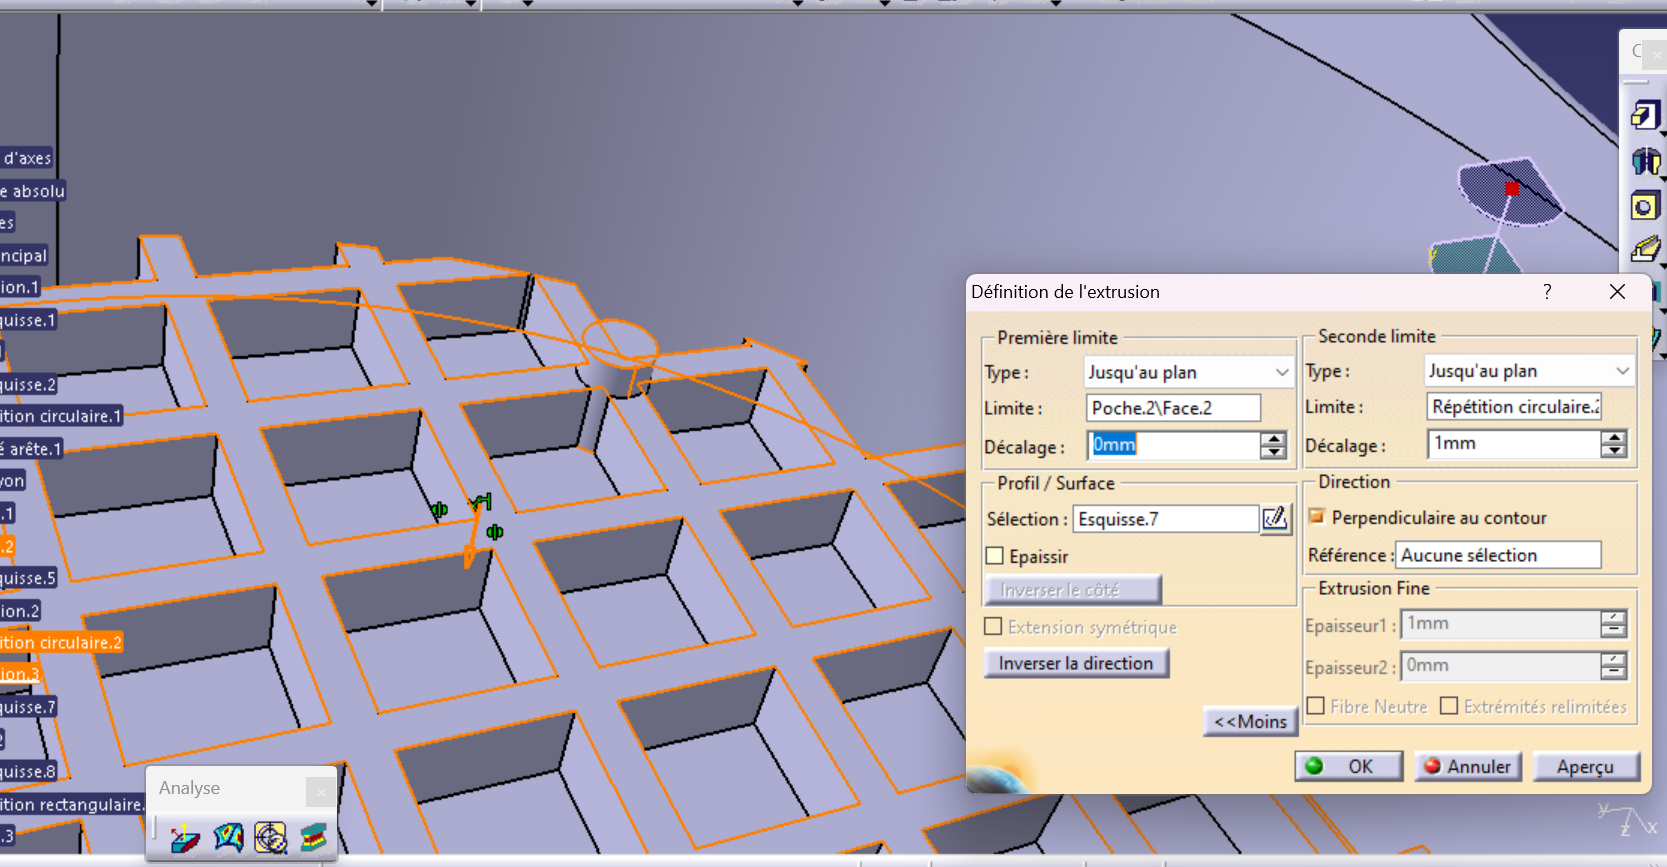
\includegraphics[width=0.8\textwidth]{images/supports_fixation_couvercle.png}
        \caption{Création des supports pour la fixation du couvercle au châssis}
        \label{fig:supports_fixation}
    \end{figure}
    
    \item \textbf{Création des taraudages pour le couvercle}:
    \begin{itemize}
        \item Utilisation de la fonction Trou (Hole) avec l'option Taraudé
        \item Type de taraudage: Métrique à pas épais
        \item Référence de taraudage: M1.6
        \item Diamètre avant trou: 1,221mm
        \item Profondeur de taraudage: 6mm
        \item Profondeur de trou: 6mm
        \item Pas: 0,35mm
        \item Option "Pas droit" sélectionnée
        \item Ces taraudages permettront de fixer solidement le couvercle protégeant l'électronique
    \end{itemize}
    
    \begin{figure}[H]
        \centering
        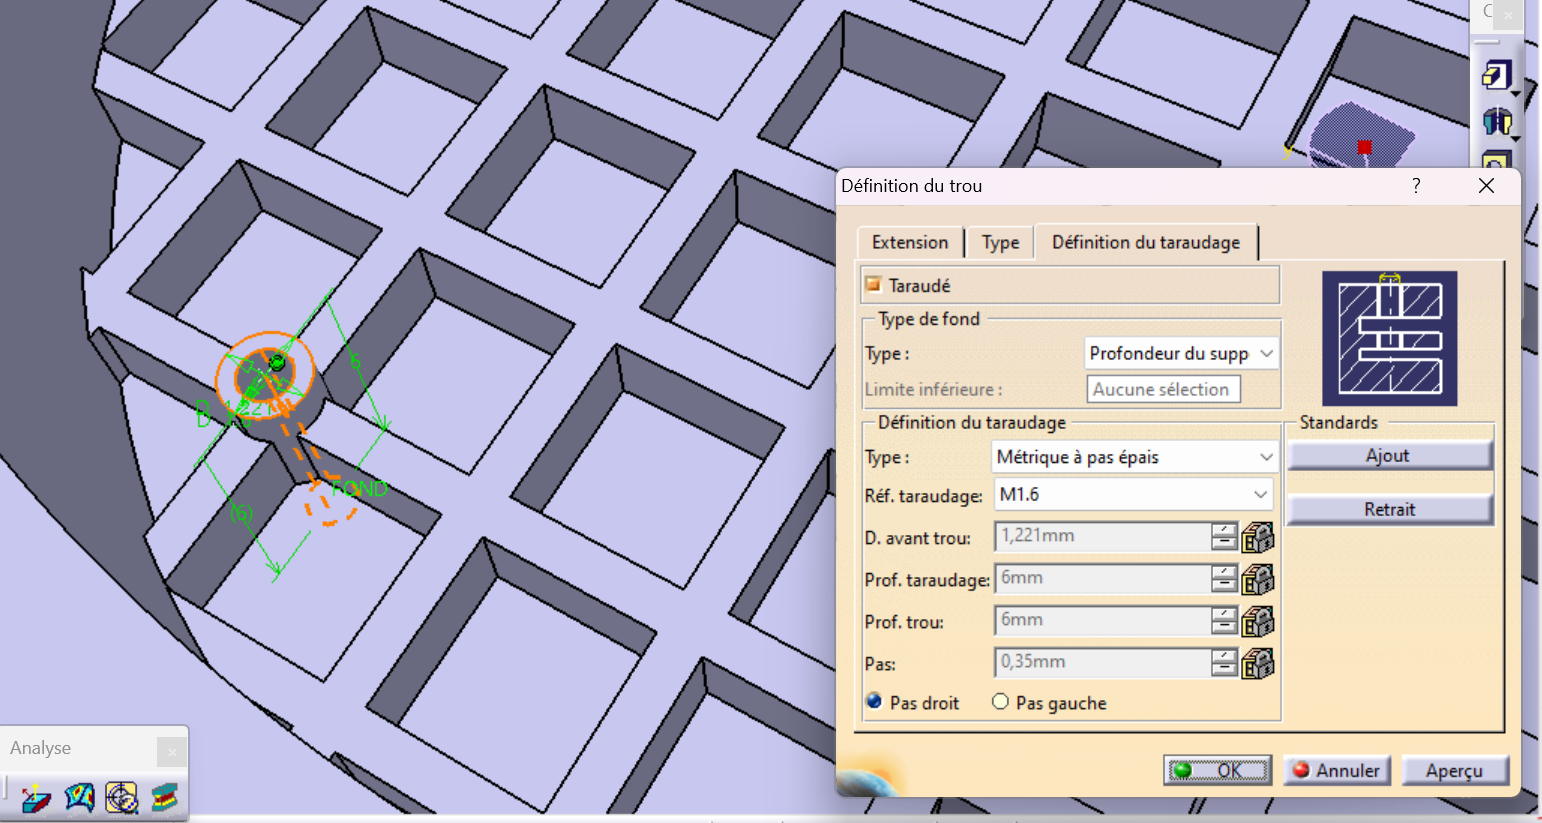
\includegraphics[width=0.8\textwidth]{images/taraudage_couvercle.png}
        \caption{Création des taraudages M1.6 pour la fixation du couvercle}
        \label{fig:taraudage_couvercle}
    \end{figure}
    
    \item \textbf{Répétition rectangulaire des taraudages}:
    \begin{itemize}
        \item Application d'un pattern rectangulaire (Rectangular Pattern) aux taraudages
        \item Composant à copier: Trou.2 (taraudage M1.6 initial)
        \item Paramètres: Instances \& espacement
        \item Première direction: 2 instances avec un espacement de 25mm
        \item Longueur totale: 25mm
        \item Élément de référence: Repère absolu\Axe
        \item Cette répétition crée un ensemble de taraudages uniformément répartis
        \item Les points de fixation aux quatre coins garantissent une fermeture stable du couvercle
    \end{itemize}
    
    \begin{figure}[H]
        \centering
        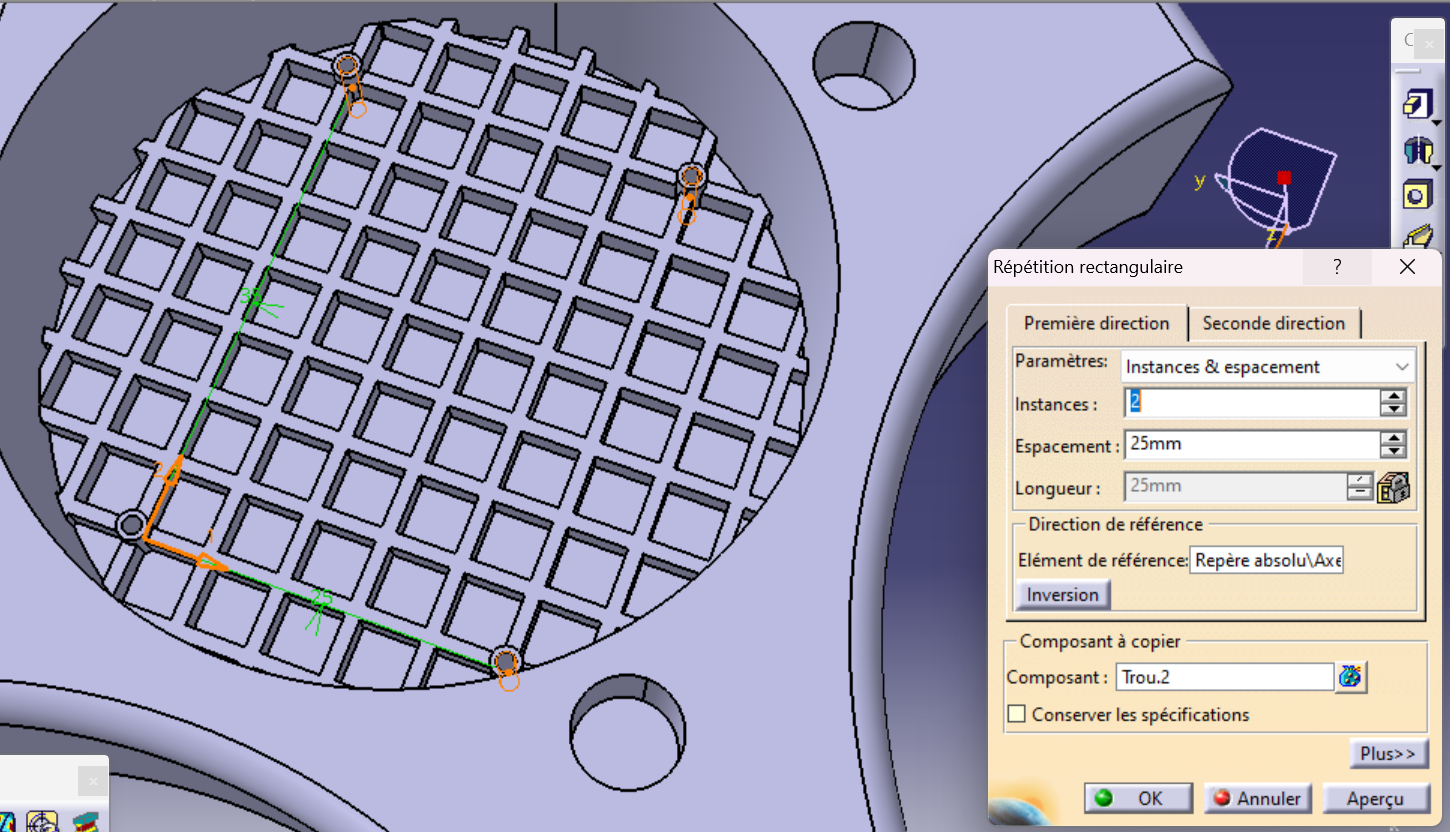
\includegraphics[width=0.8\textwidth]{images/repetition_taraudages.png}
        \caption{Répétition rectangulaire des taraudages pour la fixation du couvercle}
        \label{fig:repetition_taraudages}
    \end{figure}
    
    \item \textbf{Création du logement pour le centrage du couvercle}:
    \begin{itemize}
        \item Création d'une nouvelle esquisse (Esquisse.10) sur la face supérieure du châssis
        \item Dessin d'un cercle concentrique définissant le contour du couvercle
        \item Utilisation de la fonction Poche (Pocket) pour créer un léger rebord
        \item Profondeur de la poche: 2mm
        \item Type: Longueur (type de limite standard)
        \item Ce rebord circulaire servira à positionner et centrer précisément le couvercle
        \item Il permettra également d'assurer l'étanchéité de la zone des composants électroniques
    \end{itemize}
    
    \begin{figure}[H]
        \centering
        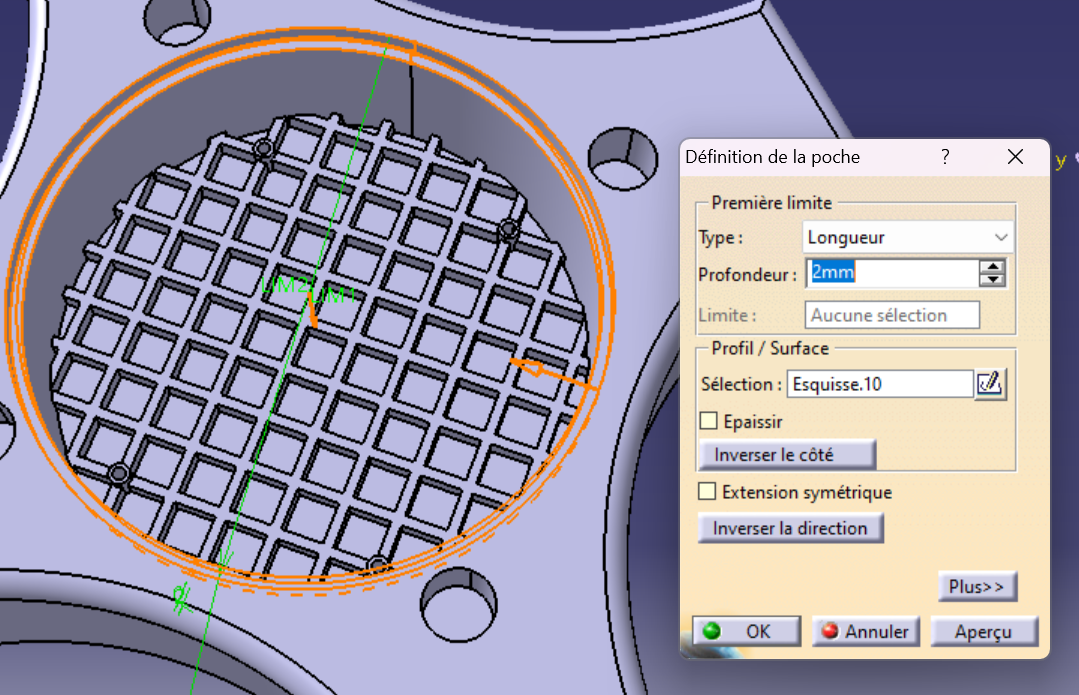
\includegraphics[width=0.8\textwidth]{images/logement_couvercle.png}
        \caption{Création du logement circulaire pour le centrage du couvercle de protection}
        \label{fig:logement_couvercle}
    \end{figure}
    
    \item \textbf{Finalisation du châssis central}:
    \begin{itemize}
        \item Le châssis central est maintenant terminé avec toutes ses fonctionnalités intégrées
        \item La pièce finale comprend les éléments suivants :
        \begin{itemize}
            \item Un corps principal extrudé de 20mm d'épaisseur
            \item Quatre trous taraudés M8 pour la fixation des bras, disposés à 90° d'intervalle
            \item Des congés de 2mm sur les arêtes extérieures pour améliorer l'ergonomie et la résistance
            \item Des poches pour la fixation des pieds du drone
            \item Une cavité centrale pour loger les composants électroniques
            \item Une structure de renforcement en quadrillage pour optimiser le rapport résistance/poids
            \item Des points de fixation avec taraudages M1.6 pour le couvercle de protection
            \item Un rebord circulaire de 2mm de profondeur pour le centrage précis du couvercle
        \end{itemize}
        \item Cette pièce centrale constitue le cœur structurel du drone, intégrant harmonieusement les fonctions mécaniques et les considérations d'assemblage
    \end{itemize}
\end{enumerate}

\begin{figure}[H]
    \centering
    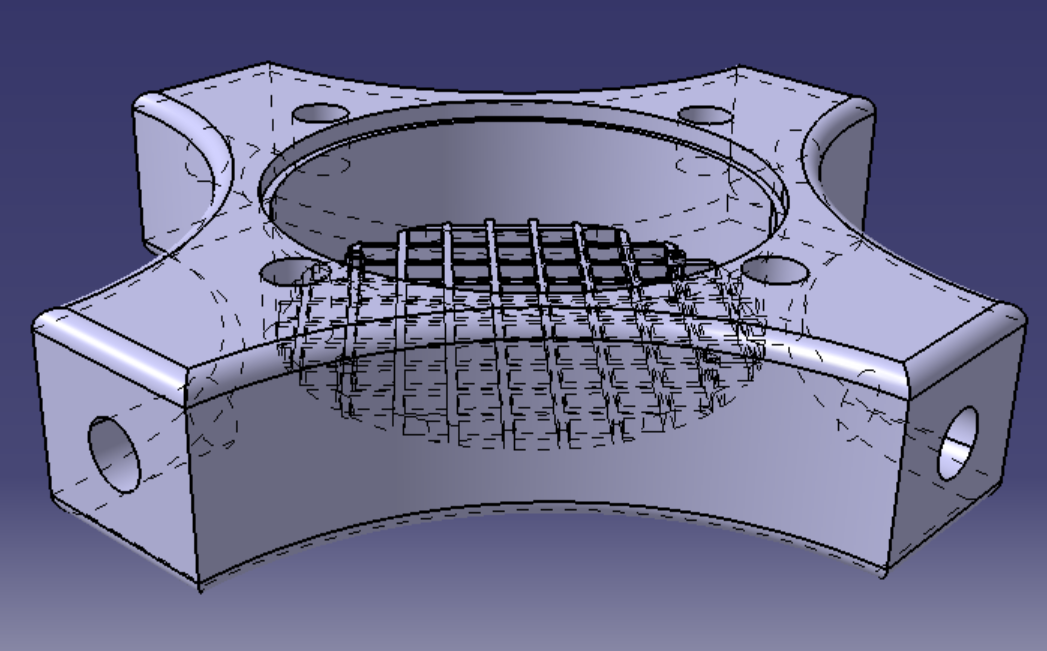
\includegraphics[width=0.7\textwidth]{images/chassis_central_final.png}
    \caption{Vue du châssis central finalisé du drone}
    \label{fig:chassis_final}
\end{figure}

\subsection{Modélisation des bras de support}
Pour modéliser les bras qui supportent les moteurs, nous avons procédé comme suit:
\begin{enumerate}
    \item \textbf{Modélisation du tube de liaison}:
    \begin{itemize}
        \item Création d'une esquisse (Esquisse.2) avec deux cercles concentriques
        \item Cercle extérieur de diamètre 10mm
        \item Cercle intérieur de diamètre 8mm (épaisseur de paroi de 1mm)
        \item Utilisation de la fonction Extrusion (Pad) pour créer le corps cylindrique
        \item Longueur d'extrusion: 30mm avec l'option d'extension symétrique activée
        \item Longueur totale obtenue: 60mm (30mm de chaque côté du plan d'esquisse)
        \item Le profil tubulaire permet un excellent rapport résistance/poids
        \item L'aluminium a été choisi pour sa légèreté et sa bonne résistance mécanique
    \end{itemize}
    
    \begin{figure}[H]
        \centering
        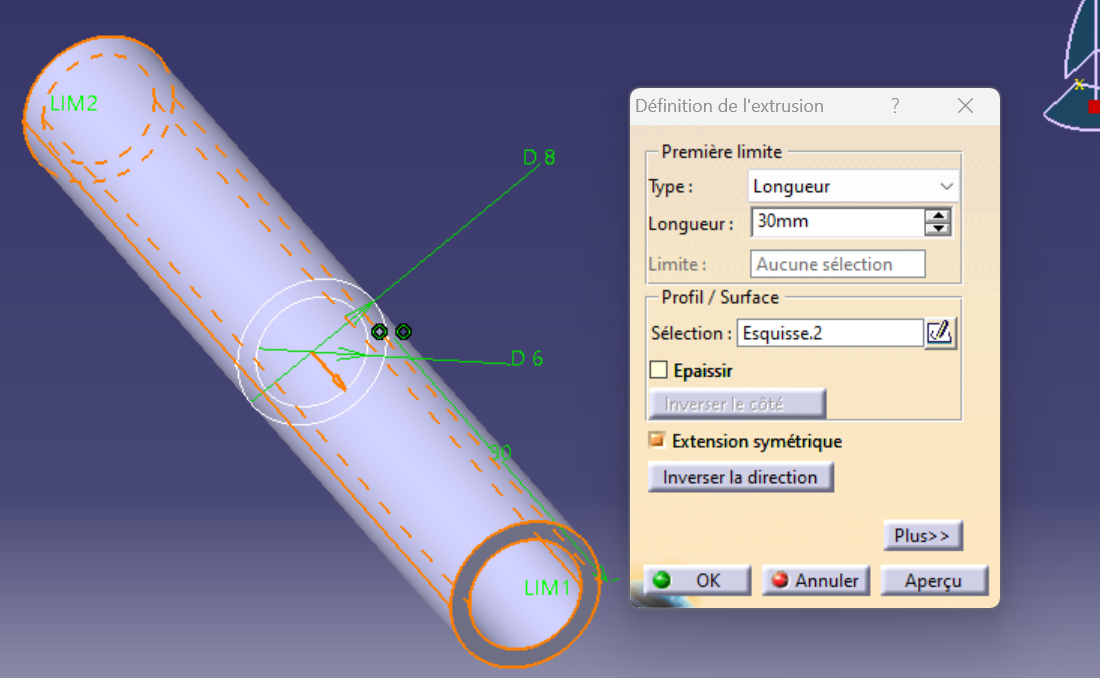
\includegraphics[width=0.7\textwidth]{images/extrusion_tube.png}
        \caption{Extrusion symétrique du profil tubulaire (30mm de chaque côté)}
        \label{fig:extrusion_tube}
    \end{figure}
    
    \item \textbf{Création des fixations hélicoïdales}:
    \begin{itemize}
        \item Ajout de filetages aux extrémités du tube pour la fixation
        \item Utilisation de la fonction filetage/taraudage (Thread/Tap) intégrée à CATIA V5
        \item Sélection de l'option "Filetage" (au lieu de "Taraudage")
        \item Définition géométrique:
        \begin{itemize}
            \item Face latérale: Extrusion.1\Face.1
            \item Face limite: Extrusion.1\Face.3
        \end{itemize}
        \item Définition numérique du filetage:
        \begin{itemize}
            \item Type: Métrique pas gros
            \item Référence: M8
            \item Diamètre du support: 8mm (diamètre intérieur du tube)
            \item Profondeur de taraudage: 10mm
            \item Hauteur du support: 60mm (longueur totale du tube)
            \item Pas: 1,25mm
            \item Option "Pas droit" sélectionnée
        \end{itemize}
        \item Ce filetage est créé sur les deux extrémités du tube
        \item Avantages de cette solution:
        \begin{itemize}
            \item Liaison solide et précise avec le châssis et le support moteur
            \item Facilité de montage/démontage pour la maintenance
            \item Résistance optimale aux vibrations des moteurs
            \item Design minimaliste sans pièces supplémentaires
        \end{itemize}
    \end{itemize}
    
    \begin{figure}[H]
        \centering
        \includegraphics[width=0.7\textwidth]{images/filetage_tube.png}
        \caption{Création du filetage M8 aux extrémités du tube de liaison}
        \label{fig:filetage_tube}
    \end{figure}
    
    \item \textbf{Finalisation du tube de liaison}:
    \begin{itemize}
        \item Le tube de liaison est maintenant terminé, prêt à être intégré dans l'assemblage
        \item Caractéristiques principales de cette pièce:
        \begin{itemize}
            \item Structure tubulaire en aluminium offrant un excellent rapport résistance/poids
            \item Diamètre extérieur de 10mm et intérieur de 8mm (épaisseur de paroi de 1mm)
            \item Longueur totale de 60mm permettant l'écartement optimal des moteurs
            \item Filetages M8 (pas 1,25mm) aux deux extrémités pour la connexion avec les autres pièces
            \item Passage interne pour les câbles électriques des moteurs
        \end{itemize}
        \item Cette conception minimaliste remplit parfaitement les objectifs d'allègement de la structure tout en maintenant la rigidité nécessaire pour un drone performant
    \end{itemize}
\end{enumerate}

\begin{figure}[H]
    \centering
    \includegraphics[width=0.7\textwidth]{images/tube_liaison_final.png}
    \caption{Vue du tube de liaison finalisé avec ses filetages aux extrémités}
    \label{fig:tube_liaison_final}
\end{figure}

Cette pièce de liaison constitue un élément essentiel dans l'architecture du drone, permettant de relier le châssis central aux supports moteurs de façon légère et robuste. Sa conception tubulaire avec filetages intégrés illustre parfaitement l'approche d'optimisation mécanique nécessaire dans le domaine des drones, où chaque gramme économisé permet d'augmenter l'autonomie de vol.

\subsection{Modélisation des supports de moteur}
Pour modéliser les supports de moteur qui servent d'interface entre les bras et les moteurs, nous avons procédé comme suit:
\begin{enumerate}
    \item \textbf{Création d'une esquisse sur le plan supérieur du bras}:
    \begin{itemize}
        \item Dessin d'un cercle de diamètre 30mm centré sur l'extrémité du bras
        \item Application des contraintes de concentricité avec l'axe central du bras
    \end{itemize}
    
    \item \textbf{Extrusion (Pad) de l'esquisse}:
    \begin{itemize}
        \item Extrusion de 5mm dans la direction Z positif
    \end{itemize}
    
    \item \textbf{Création de l'évidement central}:
    \begin{itemize}
        \item Esquisse d'un cercle de diamètre 15mm pour le passage de l'axe du moteur
        \item Création d'une poche (Pocket) traversante
    \end{itemize}
    
    \item \textbf{Création des points de fixation}:
    \begin{itemize}
        \item Esquisse de quatre cercles de 2mm de diamètre disposés en carré
        \item Espacés de 19mm selon la norme de montage des moteurs brushless
        \item Création de trous traversants (Hole) avec fraisages pour les têtes de vis
    \end{itemize}
    
    \item \textbf{Création des renforts}:
    \begin{itemize}
        \item Esquisse de trois nervures triangulaires sur la face inférieure
        \item Extrusion de 3mm pour renforcer la connexion au bras
    \end{itemize}
    
    \item \textbf{Finitions}:
    \begin{itemize}
        \item Application de congés de rayon 1mm sur toutes les arêtes exposées
        \item Chanfreins de 0.5x45° autour des trous de fixation
    \end{itemize}
\end{enumerate}

\begin{figure}[H]
    \centering
    \includegraphics[width=0.7\textwidth]{images/support_moteur.png}
    \caption{Vue 3D d'un support de moteur}
    \label{fig:support_moteur}
\end{figure}

\subsection{Modélisation des hélices}
Pour modéliser les hélices de couleur bleue, nous avons procédé comme suit:
\begin{enumerate}
    \item \textbf{Création d'une esquisse sur le plan XY}:
    \begin{itemize}
        \item Dessin d'un cercle central de diamètre 6mm pour la fixation au moteur
        \item Tracé du profil d'une pale avec une courbe spline
        \item Application des contraintes d'angle et de symétrie
    \end{itemize}
    
    \item \textbf{Extrusion (Pad) du moyeu central}:
    \begin{itemize}
        \item Extrusion du cercle central sur 5mm
    \end{itemize}
    
    \item \textbf{Création du volume des pales}:
    \begin{itemize}
        \item Utilisation de la fonction Loft (lissage) entre deux profils 
        \item Application d'un angle de torsion de 15° pour l'aérodynamisme
    \end{itemize}
    
    \item \textbf{Finitions}:
    \begin{itemize}
        \item Application d'un congé sur les bords d'attaque et de fuite des pales
        \item Réalisation d'un trou central pour la fixation sur l'axe du moteur
    \end{itemize}
    
    \item \textbf{Duplication}:
    \begin{itemize}
        \item Utilisation de la fonction de symétrie (Mirror) pour créer la deuxième pale
        \item Création des deux autres hélices avec sens de rotation inversé
    \end{itemize}
    
    \item \textbf{Application du matériau}:
    \begin{itemize}
        \item Application d'un matériau plastique léger
        \item Attribution de la couleur bleue (propriété visible sur l'image)
    \end{itemize}
\end{enumerate}

\begin{figure}[H]
    \centering
    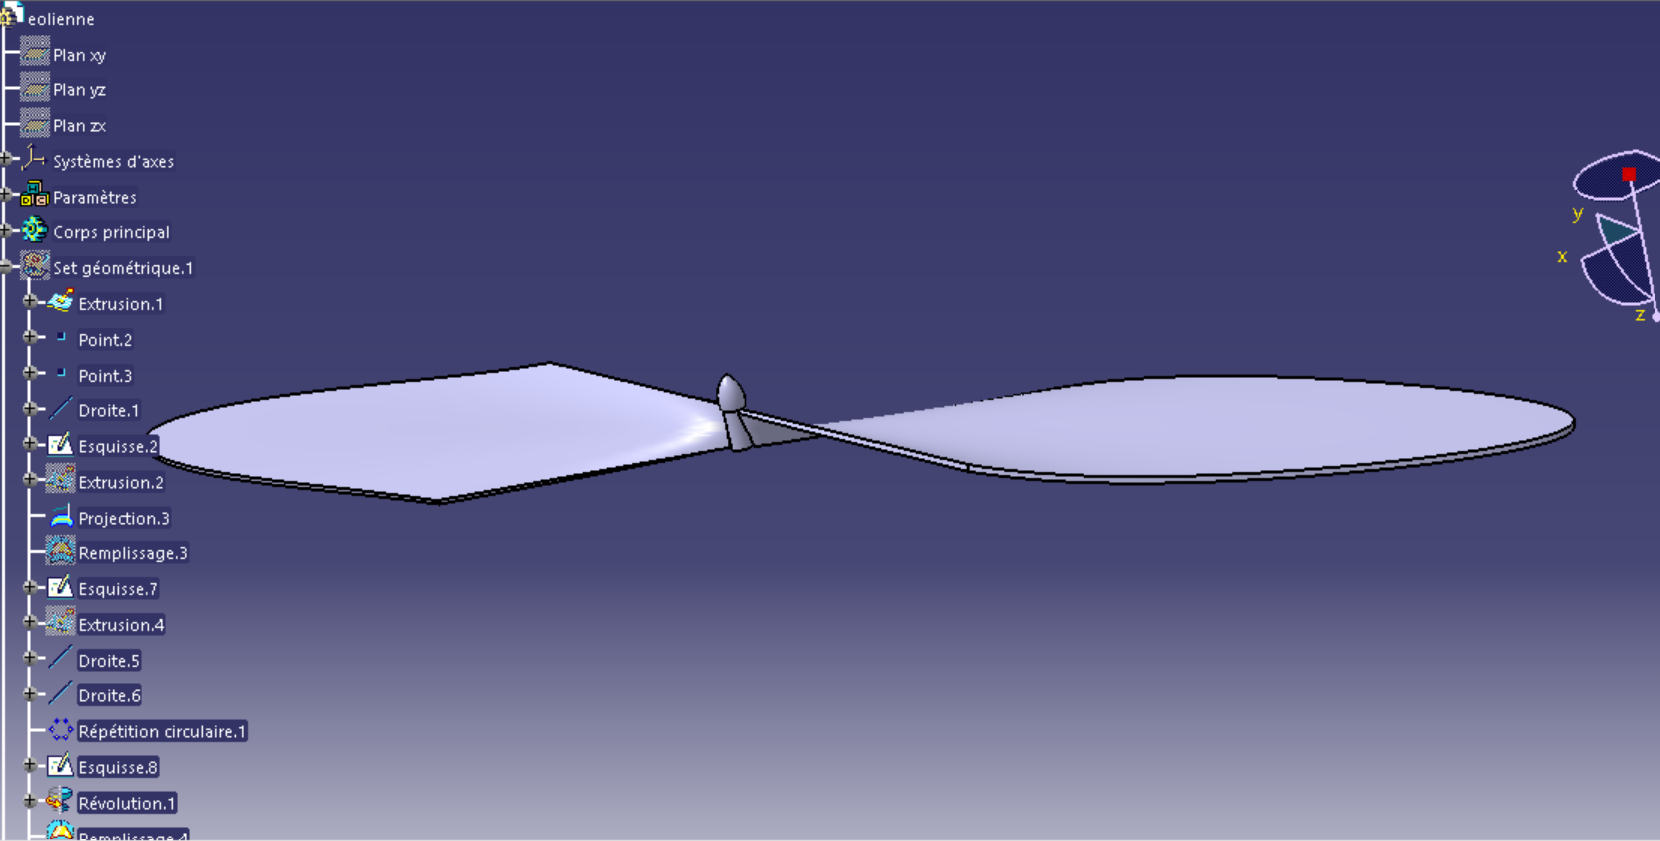
\includegraphics[width=0.7\textwidth]{images/helice_drone.png}
    \caption{Vue 3D d'une hélice}
    \label{fig:helice}
\end{figure}

\subsection{Modélisation du support d'attache}
Pour modéliser le support d'attache rouge visible sous le châssis, nous avons suivi les étapes suivantes:
\begin{enumerate}
    \item \textbf{Création d'une esquisse sur le plan XY}:
    \begin{itemize}
        \item Dessin d'une forme ergonomique adaptée à la prise en main
        \item Tracé d'une courbe fermée avec des arcs tangents
        \item Application des contraintes de symétrie par rapport à l'axe Y
    \end{itemize}
    
    \item \textbf{Extrusion (Pad) de l'esquisse}:
    \begin{itemize}
        \item Extrusion de 10mm dans la direction Z négatif
    \end{itemize}
    
    \item \textbf{Création des pattes de fixation}:
    \begin{itemize}
        \item Esquisse de deux rectangles de 10×5mm aux extrémités
        \item Extrusion de 20mm pour former les pattes de fixation
    \end{itemize}
    
    \item \textbf{Création des trous de fixation}:
    \begin{itemize}
        \item Perçage de trous de diamètre 3mm à travers les pattes
        \item Alignement des trous avec ceux du châssis central
    \end{itemize}
    
    \item \textbf{Finitions}:
    \begin{itemize}
        \item Application de congés de rayon 3mm sur toutes les arêtes
        \item Création d'une texture antidérapante sur la surface de préhension
    \end{itemize}
    
    \item \textbf{Application du matériau}:
    \begin{itemize}
        \item Application d'un matériau caoutchouc souple
        \item Attribution de la couleur rouge pour une meilleure visibilité
    \end{itemize}
\end{enumerate}

\begin{figure}[H]
    \centering
    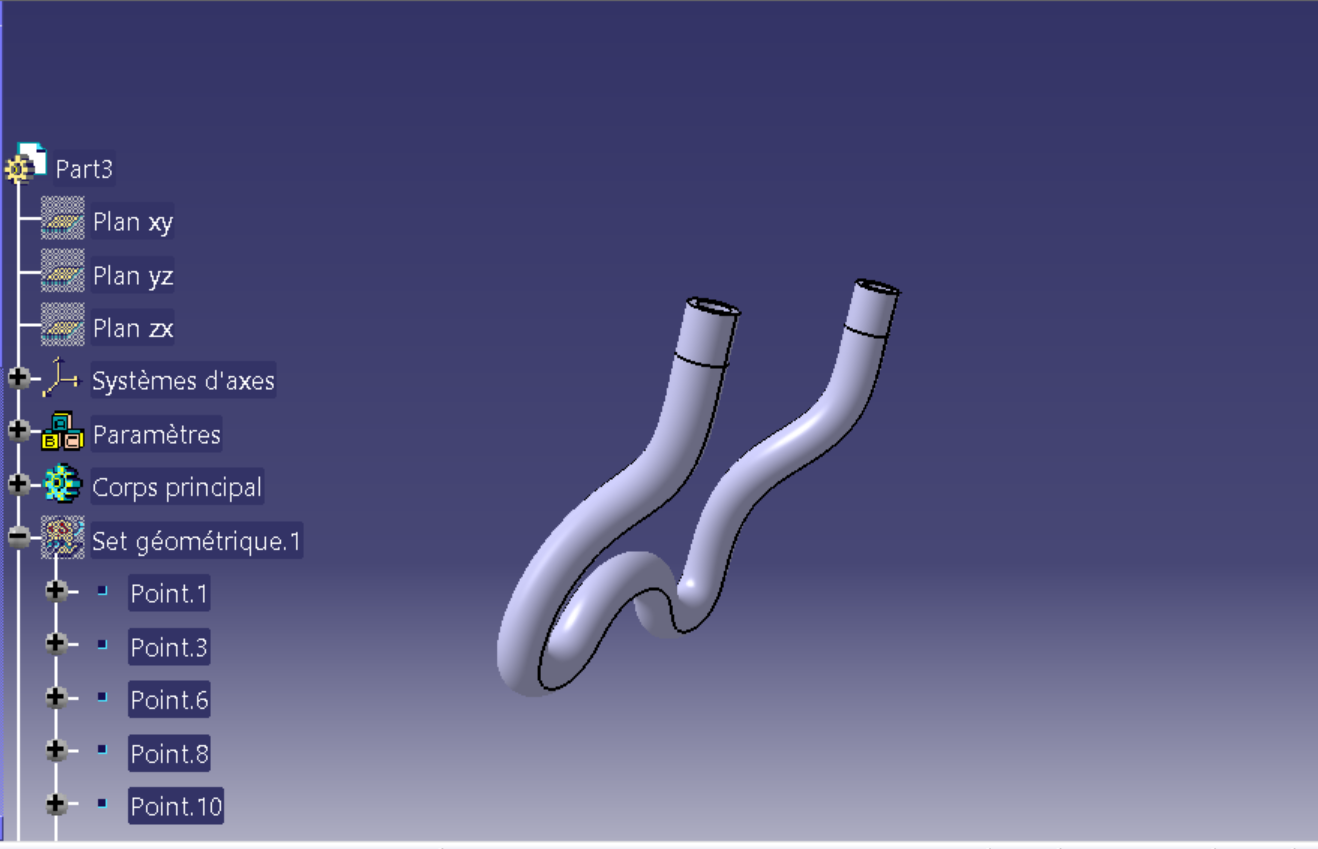
\includegraphics[width=0.7\textwidth]{images/support_attache_rouge.png}
    \caption{Vue 3D du support d'attache}
    \label{fig:support}
\end{figure}

\subsection{Modélisation des éléments de fixation}
Pour assurer l'assemblage solide des différentes pièces du drone, nous avons modélisé les éléments de fixation suivants:
\begin{enumerate}
    \item \textbf{Vis de fixation des bras au châssis}:
    \begin{itemize}
        \item Modélisation de vis M3×10 à tête fraisée
        \item Création des fraisages correspondants dans les bras
        \item Modélisation des trous taraudés dans le châssis
    \end{itemize}
    
    \item \textbf{Vis de fixation des supports de moteur}:
    \begin{itemize}
        \item Modélisation de vis M3×8 à tête cylindrique
        \item Création des logements pour les têtes de vis
        \item Modélisation des trous traversants et des taraudages
    \end{itemize}
    
    \item \textbf{Vis de fixation des moteurs}:
    \begin{itemize}
        \item Modélisation de vis M2×8 à tête cylindrique
        \item Positionnement selon la norme de fixation des moteurs brushless
        \item Création des trous traversants dans les supports de moteur
    \end{itemize}
    
    \item \textbf{Système de fixation des hélices}:
    \begin{itemize}
        \item Modélisation d'écrous autobloquants M6
        \item Création des empreintes pour assurer le serrage
        \item Modélisation des rondelles de blocage
    \end{itemize}
\end{enumerate}

Ces éléments de fixation ont été modélisés avec un niveau de détail suffisant pour assurer la cohérence de l'assemblage tout en évitant de surcharger inutilement le modèle.

\begin{figure}[H]
    \centering
    \includegraphics[width=0.7\textwidth]{images/elements_fixation.png}
    \caption{Vue des principaux éléments de fixation}
    \label{fig:fixations}
\end{figure}

\chapter{Assemblage}
\section{Structure de l'assemblage}
L'assemblage complet du drone quadrirotor est composé de 3 sous-ensembles:
\begin{itemize}
    \item \textbf{Sous-ensemble 1: Châssis et structure porteuse}
    \begin{itemize}
        \item Châssis central (corps principal)
        \item Bras de support (4 pièces)
        \item Système de fixation des bras
        \item Capot de protection électronique
    \end{itemize}
    
    \item \textbf{Sous-ensemble 2: Système de propulsion}
    \begin{itemize}
        \item Moteurs brushless (4 pièces)
        \item Hélices (4 pièces)
        \item Contrôleurs électroniques (représentés schématiquement)
    \end{itemize}
    
    \item \textbf{Sous-ensemble 3: Accessoires}
    \begin{itemize}
        \item Support d'attache (pièce rouge)
        \item Système de fixation pour accessoires
    \end{itemize}
\end{itemize}

\section{Contraintes d'assemblage}
Pour réaliser l'assemblage du drone, nous avons utilisé les contraintes suivantes:

\begin{itemize}
    \item \textbf{Contraintes de positionnement du châssis}:
    \begin{itemize}
        \item Fixation du châssis central comme pièce de référence
        \item Positionnement dans le plan XY avec l'axe Z représentant la hauteur
    \end{itemize}
    
    \item \textbf{Contraintes des bras de support}:
    \begin{itemize}
        \item Contrainte de coïncidence entre les trous de fixation des bras et ceux du châssis
        \item Contrainte de contact entre la face inférieure des bras et la face supérieure du châssis
        \item Contrainte angulaire pour l'espacement régulier à 90° entre chaque bras
    \end{itemize}
    
    \item \textbf{Contraintes des moteurs}:
    \begin{itemize}
        \item Contrainte de coïncidence entre l'axe du moteur et l'axe du trou dans le support de moteur
        \item Contrainte de contact entre la base du moteur et la face du support moteur
        \item Contrainte angulaire pour l'orientation correcte des points de fixation
    \end{itemize}
    
    \item \textbf{Contraintes des supports de moteur}:
    \begin{itemize}
        \item Contrainte de coïncidence entre l'axe du support et l'axe de l'extrémité du bras
        \item Contrainte de contact entre la face inférieure du support et la face supérieure du bras
        \item Contrainte d'alignement des trous de fixation entre le support et le bras
    \end{itemize}
    
    \item \textbf{Contraintes des hélices}:
    \begin{itemize}
        \item Contrainte de coïncidence entre l'axe de l'hélice et l'axe du moteur
        \item Contrainte de distance pour le positionnement en hauteur
        \item Contrainte d'orientation pour les sens de rotation opposés (horaire/anti-horaire)
    \end{itemize}
    
    \item \textbf{Contraintes du support d'attache}:
    \begin{itemize}
        \item Contrainte de coïncidence entre les trous de fixation du support et ceux du châssis
        \item Contrainte de contact entre la face supérieure du support et la face inférieure du châssis
        \item Contrainte de symétrie par rapport au plan central
    \end{itemize}
\end{itemize}

\begin{figure}[H]
    \centering
    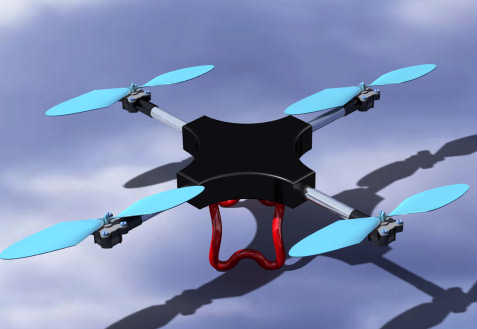
\includegraphics[width=0.8\textwidth]{images/assemblage_drone.png}
    \caption{Vue de l'assemblage complet du drone quadrirotor}
    \label{fig:assemblage}
\end{figure}

\section{Processus d'assemblage}
L'assemblage du drone a été réalisé selon les étapes suivantes:

\begin{enumerate}
    \item \textbf{Préparation du châssis central}:
    \begin{itemize}
        \item Positionnement du châssis comme pièce de référence
        \item Vérification des emplacements pour les fixations
    \end{itemize}
    
    \item \textbf{Montage des bras de support}:
    \begin{itemize}
        \item Positionnement de chaque bras dans son emplacement
        \item Fixation à l'aide des vis (représentées par les contraintes)
        \item Vérification de l'angle à 90° entre chaque bras
    \end{itemize}
    
    \item \textbf{Installation des supports de moteur}:
    \begin{itemize}
        \item Positionnement de chaque support à l'extrémité d'un bras
        \item Alignement des trous de fixation
        \item Fixation à l'aide des vis de montage
    \end{itemize}
    
    \item \textbf{Installation des moteurs}:
    \begin{itemize}
        \item Montage de chaque moteur sur son support dédié
        \item Passage des câbles d'alimentation (représentation simplifiée)
        \item Fixation à l'aide de vis (représentées par les contraintes)
    \end{itemize}
    
    \item \textbf{Montage des hélices}:
    \begin{itemize}
        \item Installation des hélices sur l'axe des moteurs
        \item Vérification de l'alternance des sens de rotation
        \item Fixation avec les écrous de serrage (simplifiés dans le modèle)
    \end{itemize}
    
    \item \textbf{Installation du support d'attache}:
    \begin{itemize}
        \item Positionnement du support sous le châssis
        \item Fixation à l'aide des vis de montage
        \item Vérification de la solidité de l'attache
    \end{itemize}
    
    \item \textbf{Vérifications finales}:
    \begin{itemize}
        \item Contrôle de l'alignement de toutes les pièces
        \item Vérification de l'absence d'interférences
        \item Test de rotation libre des hélices
    \end{itemize}
\end{enumerate}

\chapter{Dessin de définition}
\section{Cotation fonctionnelle}
Pour chaque pièce du drone, nous avons réalisé un dessin de définition avec une cotation fonctionnelle complète:

\begin{itemize}
    \item \textbf{Tolérances dimensionnelles}:
    \begin{itemize}
        \item Dimensions critiques des interfaces entre pièces: IT8
        \item Dimensions non-critiques: IT11
        \item Diamètres des trous de fixation: IT7
        \item Diamètres des emplacements des moteurs: IT9
    \end{itemize}
    
    \item \textbf{Tolérances géométriques}:
    \begin{itemize}
        \item Planéité des surfaces d'assemblage: 0,1mm
        \item Concentricité des trous pour les moteurs: 0,05mm
        \item Perpendicularité des bras par rapport au châssis: 0,2mm
        \item Symétrie des bras par rapport aux axes principaux: 0,3mm
    \end{itemize}
    
    \item \textbf{États de surface}:
    \begin{itemize}
        \item Surfaces fonctionnelles d'assemblage: Ra 3,2
        \item Surfaces visibles extérieures: Ra 1,6
        \item Surfaces intérieures non-visibles: Ra 6,3
        \item Surfaces des hélices (aérodynamiques): Ra 0,8
    \end{itemize}
\end{itemize}

\section{Mise en plan}
La mise en plan a été réalisée selon les normes ISO, avec:

\begin{itemize}
    \item \textbf{Cartouche normalisé} contenant:
    \begin{itemize}
        \item Nom de la pièce
        \item Échelle du dessin
        \item Matériau
        \item Référence
        \item Date de création
        \item Nom du concepteur
    \end{itemize}
    
    \item \textbf{Vues principales et coupes}:
    \begin{itemize}
        \item Vue de face, dessus et profil pour chaque pièce
        \item Coupes aux endroits stratégiques pour visualiser les détails internes
        \item Vues en perspective pour une meilleure compréhension
    \end{itemize}
    
    \item \textbf{Échelles adaptées}:
    \begin{itemize}
        \item Vue d'ensemble du châssis: 1:2
        \item Détails des fixations: 2:1
        \item Profil des hélices: 1:1
        \item Vue d'ensemble du drone: 1:5
    \end{itemize}
\end{itemize}

\subsection{Exemple: Dessin de définition du châssis central}
Le dessin de définition du châssis central comprend:

\begin{itemize}
    \item Vue de dessus montrant la géométrie octogonale et l'évidement central
    \item Vue en coupe A-A pour visualiser l'épaisseur des parois
    \item Détail B à l'échelle 2:1 pour les emplacements des fixations des bras
    \item Cotation complète avec:
        \begin{itemize}
            \item Diamètre externe: 160 ±0,2mm
            \item Épaisseur: 20 ±0,1mm
            \item Diamètre interne de l'évidement: 120 ±0,2mm
            \item Profondeur de l'évidement: 15 ±0,1mm
            \item Dimensions des emplacements pour les bras: 20 ±0,1mm × 10 ±0,1mm
            \item Diamètre des trous de fixation: 3 ±0,05mm
        \end{itemize}
\end{itemize}

\begin{figure}[H]
    \centering
    \includegraphics[width=0.8\textwidth]{images/dessin_chassis.png}
    \caption{Extrait du dessin de définition du châssis central}
    \label{fig:dessin_def}
\end{figure}

\subsection{Exemple: Dessin de définition des hélices}
Le dessin de définition des hélices comprend:

\begin{itemize}
    \item Vue de dessus montrant le profil complet
    \item Coupes aux différentes sections des pales pour montrer le profil aérodynamique
    \item Détail du moyeu central avec les caractéristiques de fixation
    \item Cotation complète avec:
        \begin{itemize}
            \item Diamètre total: 120 ±0,5mm
            \item Épaisseur du profil à différentes distances du centre
            \item Angle de torsion: 15° ±1°
            \item Diamètre du trou central: 6 ±0,02mm (ajustement H7)
        \end{itemize}
    \item Indications de l'état de surface aérodynamique: Ra 0,8
\end{itemize}

\begin{figure}[H]
    \centering
    \includegraphics[width=0.8\textwidth]{images/dessin_helice.png}
    \caption{Extrait du dessin de définition d'une hélice}
    \label{fig:dessin_helice}
\end{figure}

\chapter{Dessin d'ensemble}
\section{Nomenclature}
Le dessin d'ensemble du drone quadrirotor comprend une nomenclature complète avec:

\begin{itemize}
    \item \textbf{Numéro de repère}: Attribution séquentielle des numéros en commençant par le châssis
    \item \textbf{Désignation}: Nom précis de chaque composant avec référence
    \item \textbf{Matière}: Spécification des matériaux utilisés pour chaque pièce
    \item \textbf{Quantité}: Nombre d'exemplaires de chaque composant
    \item \textbf{Remarques}: Informations complémentaires sur les pièces standards ou les traitements
\end{itemize}

\begin{table}[H]
    \centering
    \caption{Extrait de la nomenclature du drone}
    \begin{tabular}{|c|l|c|c|l|}
        \hline
        \textbf{Rep.} & \textbf{Désignation} & \textbf{Matière} & \textbf{Qté} & \textbf{Observations} \\
        \hline
        1 & Châssis central & PA6 + 30\% FV & 1 & Injection plastique \\
        2 & Bras de support & PA6 + 30\% FV & 4 & Injection plastique \\
        3 & Support de moteur & PA6 + 30\% FV & 4 & Injection plastique \\
        4 & Moteur brushless & - & 4 & Réf. MT2212-920KV \\
        5 & Hélice & PVC & 4 & 2 sens horaire, 2 anti-horaire \\
        6 & Support d'attache & TPU & 1 & Matériau flexible rouge \\
        7 & Capot de protection & PC & 1 & Transparent \\
        8 & Vis de fixation bras & Acier inox & 8 & M3×10, tête fraisée \\
        9 & Vis de fixation moteur & Acier inox & 16 & M2×8, tête cylindrique \\
        10 & Écrou de fixation hélice & Laiton & 4 & M6, autobloquant \\
        11 & Vis de fixation support & Acier inox & 2 & M3×15, tête cylindrique \\
        \hline
    \end{tabular}
    \label{tab:nomenclature}
\end{table}

\section{Représentation de l'assemblage}
Le dessin d'ensemble du drone présente:

\begin{itemize}
    \item \textbf{Vue principale en coupe}:
    \begin{itemize}
        \item Coupe verticale passant par le centre du drone
        \item Visualisation de la structure interne du châssis
        \item Détail de la fixation des bras au châssis
    \end{itemize}
    
    \item \textbf{Vues complémentaires}:
    \begin{itemize}
        \item Vue de dessus complète sans coupe
        \item Vue de face avec coupe partielle
        \item Vue de dessous montrant le support d'attache
    \end{itemize}
    
    \item \textbf{Détails agrandis}:
    \begin{itemize}
        \item Détail A (2:1): Système de fixation des hélices sur les moteurs
        \item Détail B (2:1): Connexion entre les bras et le châssis
        \item Détail C (2:1): Fixation du support d'attache au châssis
    \end{itemize}
\end{itemize}

\section{Cotation d'encombrement}
Le dessin d'ensemble comprend uniquement les cotes d'encombrement principales:

\begin{itemize}
    \item Dimensions hors-tout: 380 × 380 × 120 mm (largeur × longueur × hauteur)
    \item Diamètre des hélices: 120 mm
    \item Hauteur du châssis: 20 mm
    \item Distance entre axes des moteurs opposés: 340 mm
\end{itemize}

\begin{figure}[H]
    \centering
    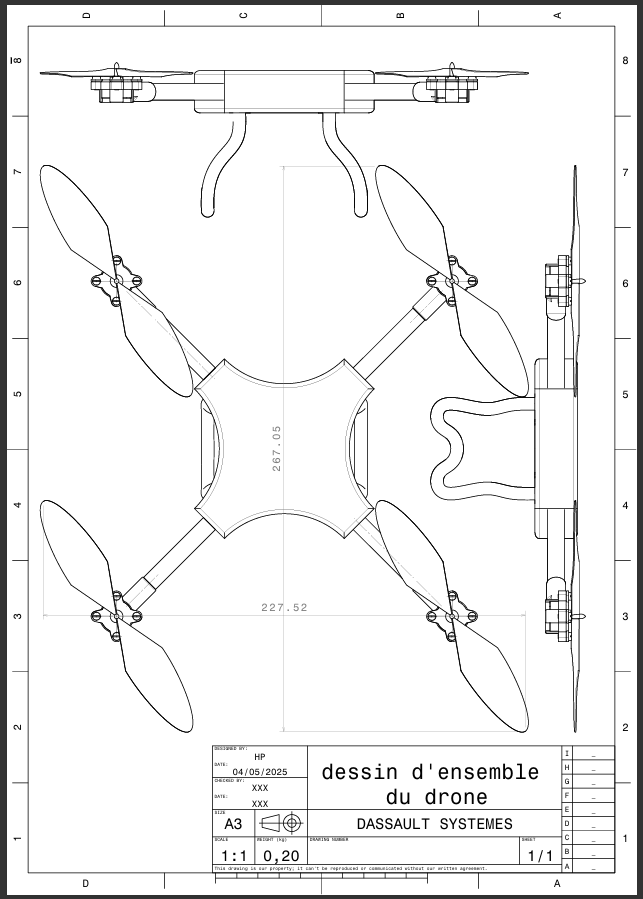
\includegraphics[width=0.8\textwidth]{images/dessin_ensemble_drone.png}
    \caption{Dessin d'ensemble du drone quadrirotor}
    \label{fig:dessin_ensemble}
\end{figure}

\section{Spécifications d'assemblage}
Le dessin d'ensemble comprend également:

\begin{itemize}
    \item \textbf{Séquence de montage numérotée}:
    \begin{enumerate}
        \item Assemblage des bras au châssis central
        \item Montage des supports de moteur aux extrémités des bras
        \item Installation des moteurs sur les supports
        \item Fixation des hélices sur les moteurs
        \item Installation du support d'attache
        \item Installation du capot de protection
    \end{enumerate}
    
    \item \textbf{Indications de couples de serrage}:
    \begin{itemize}
        \item Vis de fixation des bras: 1,2 N.m
        \item Vis de fixation des supports de moteur: 1,0 N.m
        \item Vis de fixation des moteurs: 0,8 N.m
        \item Écrous des hélices: 0,5 N.m
    \end{itemize}
    
    \item \textbf{Notes spéciales}:
    \begin{itemize}
        \item Veiller à l'orientation correcte des hélices (sens de rotation)
        \item Appliquer du frein-filet sur les écrous des hélices
        \item Vérifier l'absence d'interférence entre les hélices et la structure
    \end{itemize}
\end{itemize}

\begin{figure}[H]
    \centering
    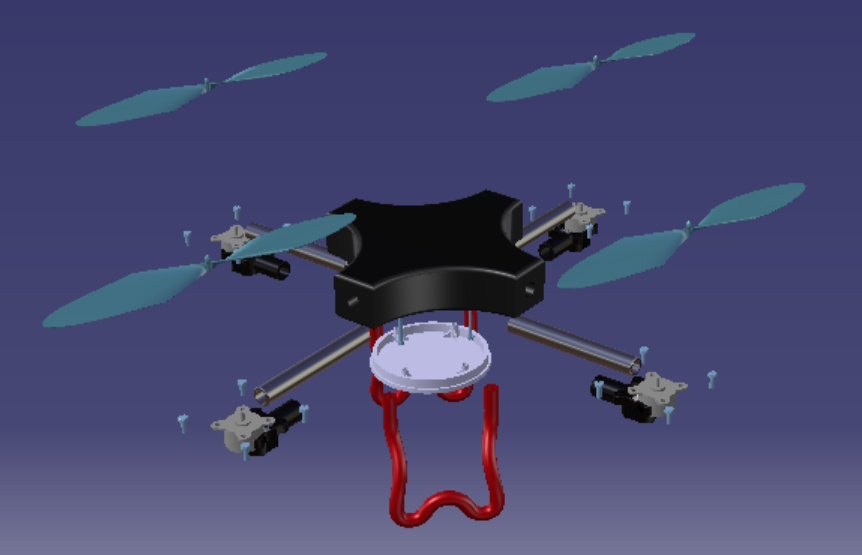
\includegraphics[width=0.8\textwidth]{images/vue_eclatee_drone.png}
    \caption{Vue éclatée du drone quadrirotor}
    \label{fig:vue_eclatee}
\end{figure}

\chapter{Analyse critique et conclusion}
\section{Difficultés rencontrées}
Au cours de ce projet de conception du drone quadrirotor, nous avons rencontré plusieurs difficultés:

\begin{itemize}
    \item \textbf{Optimisation de la géométrie du châssis}:
    \begin{itemize}
        \item La forme octogonale choisie initialement posait des problèmes d'assemblage avec les bras
        \item Difficultés pour maintenir une rigidité suffisante tout en allégeant la structure
        \item Complexité pour intégrer tous les emplacements nécessaires aux composants électroniques
    \end{itemize}
    
    \item \textbf{Conception des bras de support}:
    \begin{itemize}
        \item Compromis difficile entre légèreté et résistance mécanique
        \item Problèmes de vibrations lors des simulations des conditions de vol
        \item Difficulté d'intégration du passage des câbles d'alimentation des moteurs
    \end{itemize}
    
    \item \textbf{Modélisation des hélices}:
    \begin{itemize}
        \item Complexité du profil aérodynamique avec la torsion progressive
        \item Défi pour maintenir une géométrie identique entre les hélices de sens opposés
        \item Difficulté pour optimiser l'équilibrage des pales
    \end{itemize}
    
    \item \textbf{Assemblage et contraintes}:
    \begin{itemize}
        \item Complications dans la définition des contraintes entre les bras et le châssis
        \item Problèmes d'interférences entre les composants lors des premières tentatives d'assemblage
        \item Difficulté pour maintenir la symétrie parfaite de l'ensemble
    \end{itemize}
\end{itemize}

\section{Solutions apportées}
Pour résoudre ces difficultés, nous avons:

\begin{itemize}
    \item \textbf{Pour l'optimisation du châssis}:
    \begin{itemize}
        \item Réalisation d'une analyse par éléments finis pour identifier les zones critiques
        \item Ajout de nervures internes pour renforcer la structure sans ajouter trop de poids
        \item Utilisation d'un matériau composite (PA6 + 30\% fibres de verre) pour améliorer la rigidité
    \end{itemize}
    
    \item \textbf{Pour les bras de support}:
    \begin{itemize}
        \item Modification de la section pour une forme en I offrant une meilleure résistance à la flexion
        \item Intégration de canaux internes pour le passage des câbles
        \item Ajout de renforts aux points de jonction avec le châssis et les moteurs
    \end{itemize}
    
    \item \textbf{Pour les hélices}:
    \begin{itemize}
        \item Utilisation d'une fonction multi-sections pour mieux contrôler le profil aérodynamique
        \item Création d'un paramétrage complet permettant de générer automatiquement les hélices opposées
        \item Réalisation de simulations aérodynamiques pour optimiser la forme
    \end{itemize}
    
    \item \textbf{Pour l'assemblage}:
    \begin{itemize}
        \item Création d'un squelette d'assemblage pour garantir la symétrie
        \item Définition d'une séquence logique d'assemblage pour éviter les interférences
        \item Utilisation de contraintes paramétrées pour faciliter les modifications
    \end{itemize}
\end{itemize}

\section{Améliorations possibles}
Plusieurs améliorations pourraient être apportées à ce projet:

\begin{itemize}
    \item \textbf{Conception}:
    \begin{itemize}
        \item Intégration d'un système de protection des hélices pour plus de sécurité
        \item Optimisation topologique du châssis pour réduire davantage le poids
        \item Développement d'un mécanisme de pliage des bras pour faciliter le transport
    \end{itemize}
    
    \item \textbf{Matériaux}:
    \begin{itemize}
        \item Utilisation de matériaux plus légers comme les fibres de carbone pour certaines pièces
        \item Exploration de l'impression 3D pour des géométries plus complexes et légères
        \item Application de traitements de surface spécifiques pour améliorer la durabilité
    \end{itemize}
    
    \item \textbf{Fonctionnalités}:
    \begin{itemize}
        \item Intégration d'un système d'absorption des chocs pour les atterrissages
        \item Conception d'un compartiment étanche pour protéger l'électronique
        \item Développement d'un système de changement rapide des batteries
    \end{itemize}
\end{itemize}

\section{Conclusion}
Ce projet de conception d'un drone quadrirotor sur CATIA V5 nous a permis de développer nos compétences en conception assistée par ordinateur, notamment:

\begin{itemize}
    \item La maîtrise des fonctions avancées de modélisation 3D de CATIA V5 (extrusion, révolution, balayage, lissage)
    \item La compréhension des contraintes d'assemblage et leur application pratique
    \item L'utilisation des fonctions de mise en plan avec cotation fonctionnelle
    \item L'approche méthodique d'un projet complet, de la conception des pièces individuelles à l'assemblage final
\end{itemize}

Cette expérience nous a également sensibilisés à l'importance de l'optimisation mécanique, de la gestion des interférences et des contraintes liées à la fabrication. La réalisation de ce drone quadrirotor représente une application concrète des compétences d'ingénierie mécanique acquises durant notre formation.

Les défis rencontrés et surmontés durant ce projet constituent une préparation précieuse pour nos futures missions professionnelles, où nous serons amenés à concevoir des produits complexes en respectant des contraintes multiples.

\begin{figure}[H]
    \centering
    \includegraphics[width=0.8\textwidth]{images/drone_final.png}
    \caption{Rendu photoréaliste du drone quadrirotor finalisé}
    \label{fig:rendu_final}
\end{figure}

\end{document} 